%%%%%%%%%%%%%%%%%%%%%%%%%%%%%%%%%%%%%%%%%%%%%%%%%%%%
%%%             Metadata                         %%%
%%%%%%%%%%%%%%%%%%%%%%%%%%%%%%%%%%%%%%%%%%%%%%%%%%%%      

\title{Grundkurs Linguistik}

\subtitle{Phonetik}

\section{Phonetik}

\author[aMyP]{
	{\small Antonio Machicao y Priemer}
	\\
%	{\footnotesize \url{http://www.linguistik.hu-berlin.de/staff/amyp}\\
	{\small\href{mailto:mapriema@hu-berlin.de}{mapriema@hu-berlin.de}}
}

\institute{Institut für deutsche Sprache und Linguistik}

%%%%%%%%%%%%%%%%%%%%%%%%%      
%\date{ }
%\publishers{\textbf{6. linguistischer Methodenworkshop \\ Humboldt-Universität zu Berlin}}

%\hyphenation{nobreak}


%%%%%%%%%%%%%%%%%%%%%%%%%%%%%%%%%%%%%%%%%%%%%%%%%%%%
%%%             Preamble's End                   %%%
%%%%%%%%%%%%%%%%%%%%%%%%%%%%%%%%%%%%%%%%%%%%%%%%%%%%      


%%%%%%%%%%%%%%%%%%%%%%%%%      
\huberlintitlepage

\iftoggle{toc}{
\frame{
\begin{multicols}{2}
	\frametitle{Inhaltsverzeichnis}\tableofcontents
	%[pausesections]
\end{multicols}
}
}

%%%%%%%%%%%%%%%%%%%%%%%%%%%%%%%%%%%
%%%%%%%%%%%%%%%%%%%%%%%%%%%%%%%%%%

\nocite{Hall00a} 
\nocite{Hall00a} 
\nocite{Repp&Co12a}
\nocite{Repp&Co12a}

%%%%%%%%%%%%%%%%%%%%%%%%%%%%%%%%%%%
%%%%%%%%%%%%%%%%%%%%%%%%%%%%%%%%%%
%
\subsection{Einführung}
%\frame{
%\begin{multicols}{2}
%\frametitle{~}
%	\tableofcontents[currentsection]
%\end{multicols}
%}
%%%%%%%%%%%%%%%%%%%%%%%%%%%%%%%%%%%%%%%%%%%%%%%%
%%%%%%%%%%%%%%%%%%%%%%%%%%%%%%%%%%%%%%%%%%%%%%%%%%%%%%%%%%
\begin{frame}
	\frametitle{Begleitlektüre}
	\begin{itemize}
		\item AM S.~7--12
		\item \citet{Hall00a}: Kapitel 1 (S.~3--16; 19--31) 
	\end{itemize}
\end{frame}

%%%%%%%%%%%%%%%%%%%%%%%%%%%%%%%%%%%%%%%%%%%%%%%%%%%%


\outline{

\begin{itemize}

\item Einführung
\item Bereiche der Phonetik
\item  Methodik
\item  Probleme der Phonetik
\item  IPA-Alphabet
\item Artikulatorische Phonetik
%% Konsonanten
%% Konsonantenklassi kation
%% Vokale
%% Vokalklassi kation
%% Vokalviereck
%% Monophthong, Diphthong, Triphthong
\item Übungen
  
  \end{itemize}
}

\begin{frame}
\frametitle{Einführung}

	\begin{itemize}
		\item Phonetik $\approx$ \gqq{Lautlehre}, \gqq{Lehre der Sprachlaute}, \gqq{Sprechaktlautlehre}
		\item[]
		\item Sie beschäftigt sich mit der \textbf{materiellen Seite} des Sprechens $\rightarrow$ Sprachlaute 
		\item[]
		\item \textbf{Minimaleinheit} der Phonetik:\\
                      \textbf{Phon} $\approx$ Sprachlaut $\approx$ Segment $\approx$ einfach nur \gqq{Laut}
		\item[]
		\item Sie zählt nicht im engeren Sinne zu den \textit{grammatischen Modulen} in der Sprachkompetenz, sondern zu dem \textbf{artikulatorisch-perzeptorischen Apparat}.
	\end{itemize}
	
\end{frame}



%%%%%%%%%%%%%%%%%%%%%%%%%%%%%%%%%%%%%%%%%%%%%%%%%%%%%%%%%%%%

\begin{frame}
\frametitle{Laute in den Sprachen der Welt}

	\begin{itemize}
		\item Insgesamt zählt man über \textbf{200 Vokale} und über \textbf{500 Konsonanten}.
		
		\begin{itemize}
			\item[]
			\item Pirahã: 10 Laute (eher Phoneme)\\
			\textbf{VIDEO:} \href{run:material/04SpokenPiraha.mp4}{Spoken Pirahã with subtitles}
			\item[]
			\item Hawaiianisch: 11--13 Laute (eher Phoneme)
			\item[]
			\item {!}Xóõ: 141--159 Laute (eher Phoneme)
			\item[]
			\item Deutsch: 50 Laute (ung. 32 Phoneme)
		\end{itemize}
		
	\end{itemize}
	
\end{frame}



%%%%%%%%%%%%%%%%%%%%%%%%%%%%%%%%%%%%%%%%%%%%%%%%%%%%%%%%%%%%%%%%

\begin{frame}
\frametitle{Übung}

Wie viele Laute haben die folgenden Wörter?
		
		\begin{columns}
			\column{.30\textwidth}
				\begin{enumerate}
					\item \ab{Fische}
					\item \ab{Nixe}
					\item \ab{lang}
					\item \ab{Bearbeitung}
				\end{enumerate} 				
			\column{.35\textwidth}
				\begin{enumerate}
					\item<2> \textipa{[ f \textsci{} \textesh{} @ ]}
					\item<2> \textipa{[ n \textsci{} k s @ ]}
					\item<2> \textipa{[ l a N ]}
					\item<2> \textipa{[ b @ P a \textscr\  b \t{aI} t U N ]}
					\item<2>[] \textipa{[ b @ P a  b \t{aI} t U N ]}
				\end{enumerate} 
			\column{.15\textwidth}
				\begin{enumerate}
					\item<2>[] 4
					\item<2>[] 5
					\item<2>[] 3
					\item<2>[] 10--11 % bearbeitung ai als ein
                                          % Laut oder als zwei gezählt
					\item<2>[] 9--10 % beabeitung ai als ein
                                          % Laut oder als zwei gezählt
                \end{enumerate}
		\end{columns}


                \bigskip
                
                \textipa{\t{aI}} kann man als einen oder als zwei Laute zählen.

\end{frame}



%%%%%%%%%%%%%%%%%%%%%%%%%%%%%%%%%%%%%%%%%%%%%%%%%%%%%%%%%%%%%%%%

\begin{frame}
\frametitle{Einordnung der Phonetik als Wissenschaft}

	\begin{itemize}
	
		\item Methodik: \textbf{naturwissenschaftlich}
		\item Messung und Analyse physiologischer und physikalischer Aspekte der Sprache
		\item \textbf{Lautkontinuum} wird in einzelne Laute zerlegt
		\item[]
		\item Bereiche der Phonetik:

		\begin{itemize}
			\item Artikulatorische Phonetik
			\item[]
			\item Akustische Phonetik
			\item[]
			\item Auditive (perzeptive) Phonetik
		\end{itemize}
		
	\end{itemize}
	
\end{frame}



%%%%%%%%%%%%%%%%%%%%%%%%%%%%%%%%%%%%%%%%%%%%%%%%%%%%%%%%%%%%%%%%
%%%%%%%%%%%%%%%%%%%%%%%%%%%%%%%%%%%%%%%%%%%%%%%%%%%%%%%%%%%%%%%
%
\subsection{Bereiche der Phonetik}
%
\iftoggle{toc}{
\frame{
\begin{multicols}{2}
	\tableofcontents[currentsection]
\end{multicols}
}
}

\outline{

\begin{itemize}

\item Einführung
\item \blaubf{Bereiche der Phonetik}
  \item  Methodik
\item  Probleme der Phonetik
\item  IPA-Alphabet
\item Artikulatorische Phonetik
%% Konsonanten
%% Konsonantenklassi kation
%% Vokale
%% Vokalklassi kation
%% Vokalviereck
%% Monophthong, Diphthong, Triphthong
\item Übungen
  
  \end{itemize}
}


%%%%%%%%%%%%%%%%%%%%%%%%%%%%%%%%%%%%%%%%%%%%%%%%%%%%%%%%%%%%%%%%

\begin{frame}{Bereiche der Phonetik}

	\begin{table}
	\centering 
	
		\begin{tabular}{p{0.23\linewidth}p{0.05\linewidth}p{0.23\linewidth}p{0.05\linewidth}p{0.23\linewidth}}
			\hline
			\textbf{Artikulatorische Phonetik} & & \textbf{Akustische}\par \textbf{Phonetik} & & \textbf{Auditive}\par \textbf{(perzeptive)}\par \textbf{Phonetik} \\
			\hline
  			Sprecher & & Schallsignal & & Hörer \\
			\hline
			Lautproduktion & $\rightarrow$ & Transmission & $\rightarrow$ & Perzeption\\
			\hline
		\end{tabular}
		
	\caption{Bereiche der Phonetik \citep{Ramers08a}} 
	\end{table}	
		
\end{frame}



%%%%%%%%%%%%%%%%%%%%%%%%%%%%%%%%%%%%%%%%%%%%%%%%%%%%%%%%%%%%%%%%

\begin{frame}
\frametitle{Bereiche der Phonetik}

	\begin{itemize}
		\item \textbf{Artikulatorische Phonetik}
		
\textbf{Erzeugung} von Lautereignissen (von der Steuerung durch das Gehirn bis zu den konkreten artikulatorischen Bewegungen im Mund-, Rachen- und Nasenraum und im Kehlkopf)

			\ea Zungenbewegung bei der Aussprache des Lautes \textipa{[ \t{tS} ]}
			\z

		
		\item \textbf{Akustische Phonetik}
		
                       physikalische Eigenschaften von \textbf{Schallwellen}, die bei der Produktion und Übertragung von Sprachlauten auftreten

			\ea physikalische Eigenschaften eines Lauts im Übertragungsprozess: Frequenzbereich, Intensität, Länge, etc.
			\z
			
		\item \textbf{Auditive (perzeptive) Phonetik}
		
		      \textbf{Wahrnehmung} (Empfang und Verstehen) von Sprachlauten

			\ea Wie nimmt der Hörer den Unterschied zwischen den Vokalen in \ab{Beet} und \ab{Bett} wahr?
			\z
		
	\end{itemize}
	
\end{frame}



%%%%%%%%%%%%%%%%%%%%%%%%%%%%%%%%%%%%%%%%%%%%%%%%%%%%%%%%%%%%%%%%
%%%%%%%%%%%%%%%%%%%%%%%%%%%%%%%%%%%%%%%%%%%%%%%%%%%%%%%%%%%%%%%%
%
\subsection{Methodik}
\iftoggle{toc}{
\frame{
\begin{multicols}{2}
	\tableofcontents[currentsection]
\end{multicols}
}
}
\outline{

\begin{itemize}

\item Einführung
\item Bereiche der Phonetik
\item \blaubf{Methodik}
\item Probleme der Phonetik
\item IPA-Alphabet
\item Artikulatorische Phonetik
%% Konsonanten
%% Konsonantenklassi kation
%% Vokale
%% Vokalklassi kation
%% Vokalviereck
%% Monophthong, Diphthong, Triphthong
\item Übungen
  
  \end{itemize}
}

%%%%%%%%%%%%%%%%%%%%%%%%%%%%%%%%%%%%%%%%%%%%%%%%%%%%%%%%%%%%%%%%

\begin{frame}{Methodik}

	\begin{figure}
		\centering
		
		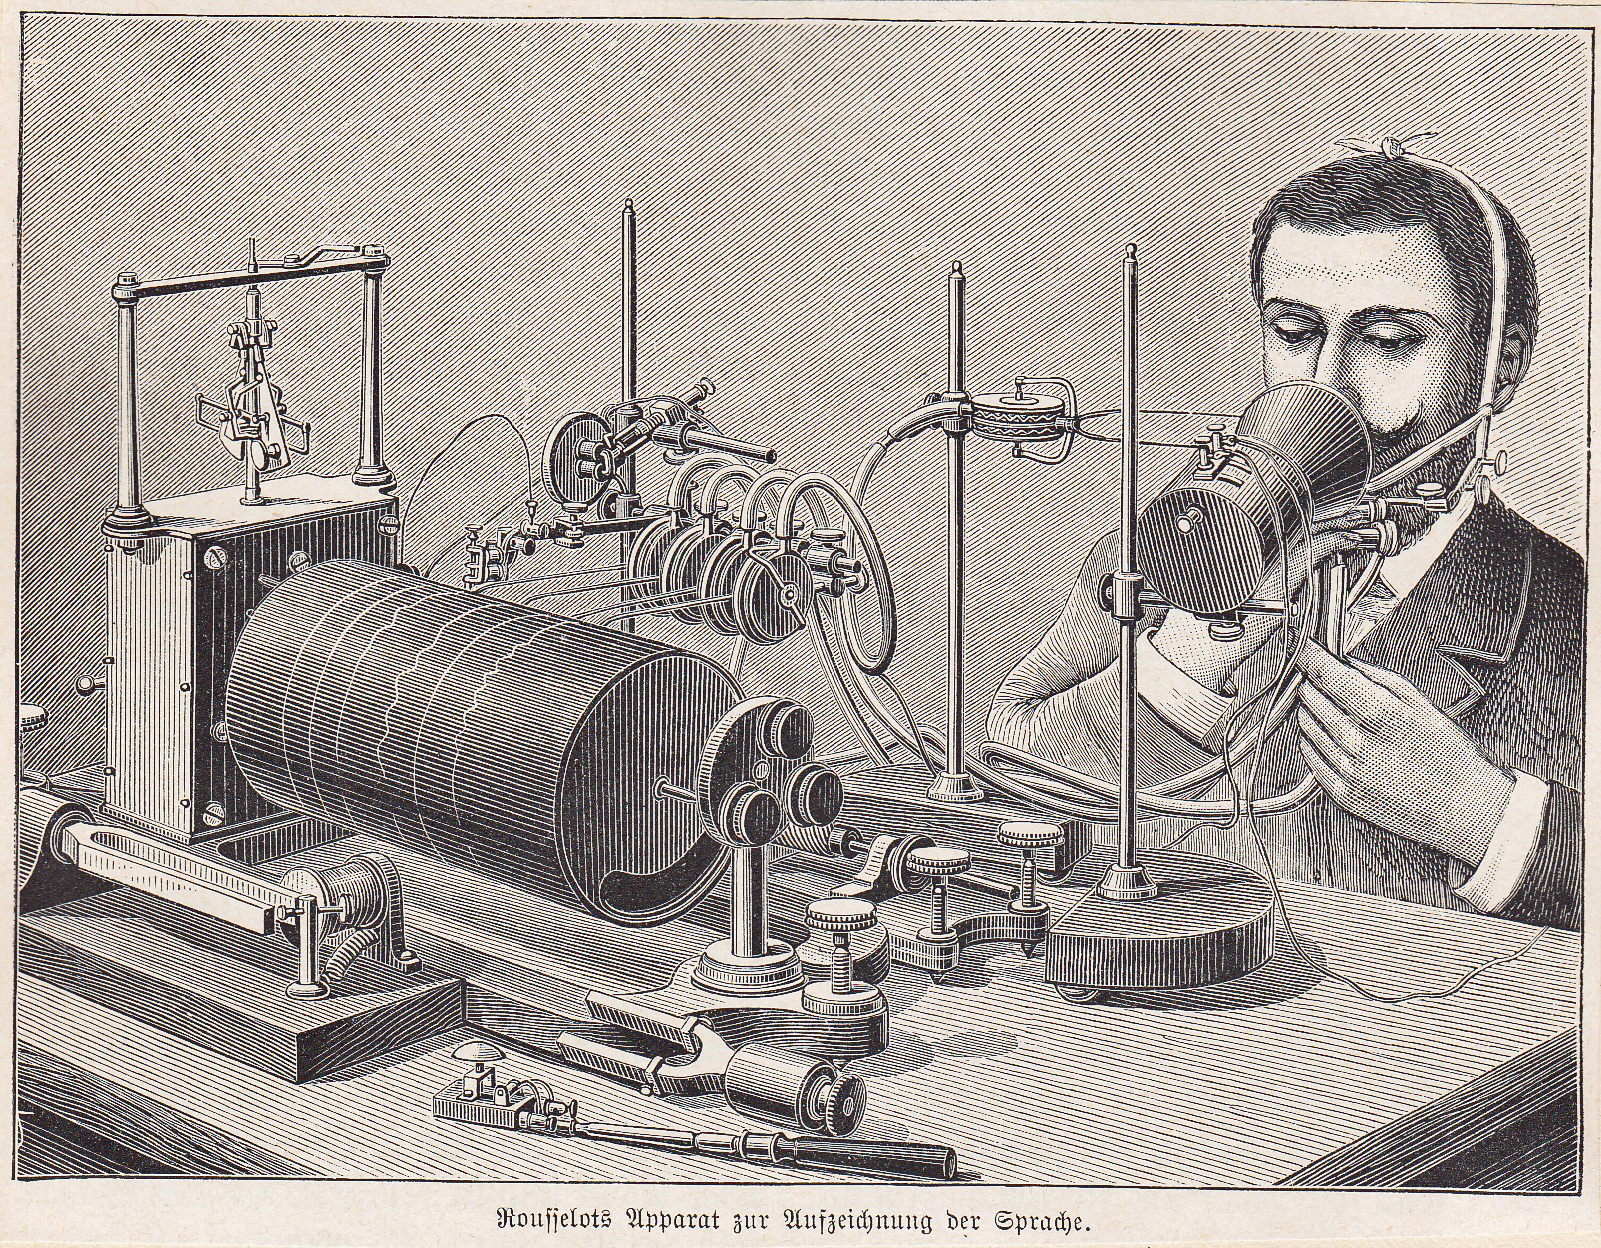
\includegraphics[scale=0.1]{material/04RousselotsApparatzurAufzeichnungderSprache}
		\caption{Rousselots Apparat zur Aufzeichnung der Sprache (Holzstich, um 1900)
}
		%{material/04proband}
		%\caption{Proband \citep{Pompino95a}}
		%\label{Zeichen1}
	\end{figure}
	
\end{frame}


%%%%%%%%%%%%%%%%%%%%%%%%%%%%%%%%%%%%%%%%%%%%%%%%%%%%%%%%%%%%%%%%

\begin{frame}
\frametitle{Deskriptive, Symbol-, Instrumental- und Signalphonetik}

	\begin{itemize}
		\item Der geschulte Ohrenphonetiker analysiert und beschreibt das Gehörte
                  (\textbf{deskriptive Phonetik}).

                  Die analysierten Lautkategorien werden anschließend mit symbolischen Mitteln (dem Internationalen Phonetischen Alphabet -- IPA) dargestellt (\textbf{Symbolphonetik}).

		\item Phonetiker nehmen die ablaufenden physikalischen Vorgänge mittels spezieller Mess- oder Registriergeräte während des Sprechaktes als Signale auf (\textbf{Instrumental-} oder \textbf{Signalphonetik}).
	\end{itemize}
	
\end{frame}



%%%%%%%%%%%%%%%%%%%%%%%%%%%%%%%%%%%%%%%%%%%%%%%%%%%%%%%%%%%%%%%%

\begin{frame}
\frametitle{Methodik: Beispiele}

	\begin{itemize}
\item Kiefer-, Lippen- und Zungenbewegungen mithilfe der elektrischen Muskelpotenziale
\item Luftdruckschwankungen, die das akustische Signal darstellen
\item Verlauf des intraoralen Luftdrucks
\item Veränderung der Durchblutung bestimmter Großhirnregionen bei der Verarbeitung von lautsprachlichen Reizen
	\end{itemize}
	
\end{frame}



%%%%%%%%%%%%%%%%%%%%%%%%%%%%%%%%%%%%%%%%%%%%%%%%%%%%%%%%%%%%%%%%

\begin{frame}
\frametitle{Experimental- und perzeptive Phonetik}

	\begin{itemize}
		\item Außerdem kann man den Zusammenhang zwischen bestimmten Signalausprägungen und
                  der Wahrnehmung von Versuchspersonen untersuchen (\textbf{Experimentalphonetik}
                  oder \textbf{perzeptive Phonetik}).

                  Damit wird ein Zusammenhang zwischen der Instrumentalphonetik und der deskriptiven Phonetik erzeugt.

                  \item Beispiel:\\
		  Bei Veränderung von einzelnen akustischen Parametern:\\
                  Ab wann nimmt eine Versuchsperson ein \textipa{[ da ]} als \textipa{[ ta ]} wahr?
	

	\end{itemize}
	
\end{frame}



%%%%%%%%%%%%%%%%%%%%%%%%%%%%%%%%%%%%%%%%%%%%%%%%%%%%%%%%%%%%%%%%
%%%%%%%%%%%%%%%%%%%%%%%%%%%%%%%%%%%%%%%%%%%%%%%%%%%%%%%%%%%%%%%%
%
\subsection{Probleme der Phonetik}
\iftoggle{toc}{
\frame{
\begin{multicols}{2}
	\tableofcontents[currentsection]
\end{multicols}
}
}

\outline{

\begin{itemize}

\item Einführung
\item Bereiche der Phonetik
\item  Methodik
\item  \blaubf{Probleme der Phonetik}
\item  IPA-Alphabet
\item Artikulatorische Phonetik
%% Konsonanten
%% Konsonantenklassi kation
%% Vokale
%% Vokalklassi kation
%% Vokalviereck
%% Monophthong, Diphthong, Triphthong
\item Übungen
  
  \end{itemize}
}


%%%%%%%%%%%%%%%%%%%%%%%%%%%%%%%%%%%%%%%%%%%%%%%%%%%%%%%%%%%%%%%%%

\begin{frame}{Probleme der Phonetik: Schnelle Übermittlung der Laute}

		\begin{itemize}
			\item kurzer Satz (mit 50 Segmenten) \ras ung. 2 Sekunden
			\item[]
			\item d.\,h. bis zu 25 (sprachliche) Segmente pro Sekunde
			\item[]
			\item nicht-sprachliche Segmente \ras ung. 7 bis 9 pro Sekunde
			\item[]
			\item[\ra] Hohe Geschwindigkeit bei der Äußerung eines Satzes macht aus einer sprachlichen Äußerung ein \textbf{Kontinuum}, in dem die Segmentierung der Laute besonders schwer ist.
		\end{itemize}
		
	
\end{frame}


%%%%%%%%%%%%%%%%%%%%%%%%%%%%%%%%%%%%%%%%%%%%%%%%%%%%%%%%%%%%%%%

\begin{frame}
\frametitle{Schallsignal ist Kontinuum, Segmentierung schwierig}

	\begin{figure}[H]
	\centering
	
	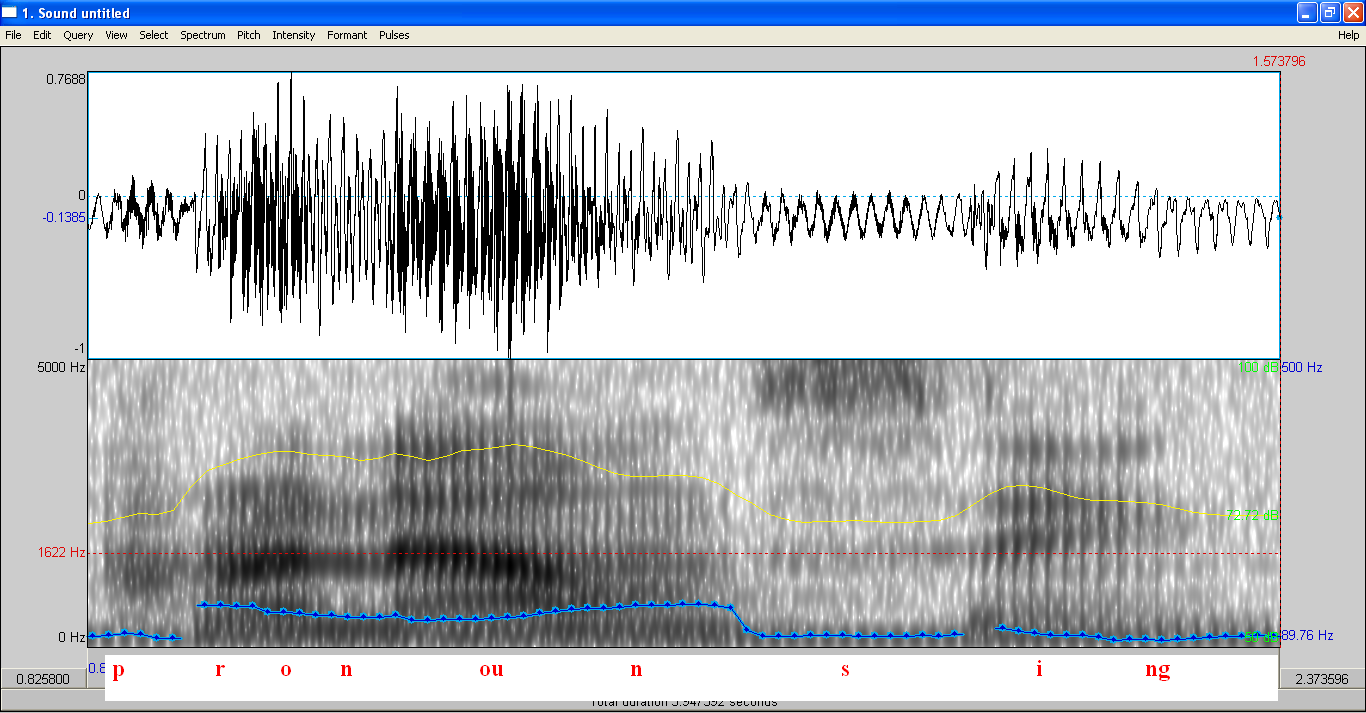
\includegraphics[scale=0.2]{material/04Pronouncing}
	\caption{Spektrogramm \emph{pronouncing}}
	%Die alte Version: \includegraphics[scale=0.50]{material/oszillogrammwiese} \caption{\citep{WieseR11a}}
	%\label{Zeichen1}
	\end{figure}	
	
\end{frame}


%%%%%%%%%%%%%%%%%%%%%%%%%%%%%%%%%%%%%%%%%%%%%%%%%%%%%%%%%%%%%%%%

\begin{frame}
\frametitlefit{Keine 1-zu-1-Korrespondenz zw.\ Lauten und Verschriftlichung}

		\begin{itemize}
			\item[]
			\item Ein Laut \ras mehrere Buchstaben

			\ea \textipa{[s]} \ras \ab{\textbf{S}maragd}, \ab{gro\textbf{ß}}, \ab{e\textbf{ss}en}
			\z
			
			\item[]
			\item Eine Buchstabenfolge \ras unterschiedliche Laute

			\ea \ab{ch} \ras \ab{mi\textbf{ch}}, \ab{Bu\textbf{ch}}, \ab{se\textbf{ch}s}, \ab{\textbf{Ch}arme}, \ab{\textbf{Ch}ip}
			\z

			\item[]
			\item[\ras] Schriftsystem mit 1-zu-1-Korrespondenz zwischen Lauten und (diakritischen) Zeichen: \textbf{IPA-Alphabet}
		\end{itemize}
		
\end{frame}


%%%%%%%%%%%%%%%%%%%%%%%%%%%%%%%%%%%%%%%%%%%%%%%%%%%%%%%%%%%%%%%%
%%%%%%%%%%%%%%%%%%%%%%%%%%%%%%%%%%%%%%%%%%%%%%%%%%%%%%%%%%%%%%%%
%
\subsection{IPA-Alphabet}
\iftoggle{toc}{
\frame{
\begin{multicols}{2}
	\tableofcontents[currentsection]
\end{multicols}
}
}
\outline{

\begin{itemize}

\item Einführung
\item Bereiche der Phonetik
\item  Methodik
\item  Probleme der Phonetik
\item  \blaubf{IPA-Alphabet}
\item Artikulatorische Phonetik
%% Konsonanten
%% Konsonantenklassi kation
%% Vokale
%% Vokalklassi kation
%% Vokalviereck
%% Monophthong, Diphthong, Triphthong
\item Übungen
  
  \end{itemize}
}

%%%%%%%%%%%%%%%%%%%%%%%%%%%%%%%%%%%%%%%%%%%%%%%%%%%%%%%%%%%%%%%%

\begin{frame}{IPA-Alphabet}

	\begin{itemize}
		\item IPA = International Phonetic Association \ras IPA-Alphabet
		\item Seit Mitte des 19. Jh. \ras Entwicklung von phonetischen Umschriftsystemen
		\item IPA-Alphabet ist das am weitesten verbreitete System.
		\item Alle Sprachlaute aller natürlichen Sprachen werden eindeutig dargestellt (phonetische Transkription).
		\item[]
		\item \textbf{Repräsentation der Phone} \ras in eckigen Klammern \gqq{\textipa{[ ]}}
		\item \textbf{Orthographische Repräsentation} \ras in spitzen Klammern \gqq{$\langle{} \rangle{}$}
		\item[]
		\item {Webseite der IPA}:\\ \url{http://internationalphoneticassociation.org}
		\item {Alle Laute zum Testen}: \url{http://phonetics.ucla.edu/course/chapter1/chapter1.html}
	\end{itemize}
	
\end{frame}


%%%%%%%%%%%%%%%%%%%%%%%%%%%%%%%%%%%%%%%%%%%%%%%%%%%%%%%%%%%%%%%%

%\begin{frame}
%\frametitle{IPA-Alphabet}
%
%	\begin{figure}[H]
%		\centering
%		
%		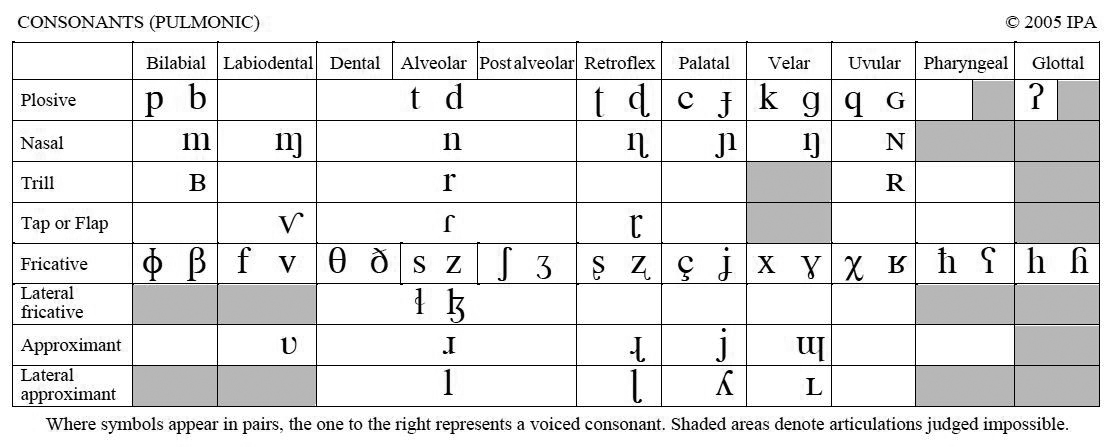
\includegraphics[scale=0.35]{material/04ipaconsonantpulmonic}
%		\caption{Konsonanten (Pulmonal)}
%		%\label{Zeichen1}
%	\end{figure}	
%	
%\end{frame}

%%%%%%%%%%%%%%%%%%%%%%%%%%%%%%%%%%%%%%%%%%%%%%%
\begin{frame}
\frametitle{Pulmonische Konsonanten im IPA-Alphabet}
\begin{table}
\centering
\begin{adjustbox}{max width=\textwidth}
\begin{tabular}{|p{0.1\textwidth}|c|c|c|c|c|c|c|c|c|c|c|c|c|}
\hline
& \tiny{Bilabial} & \tiny{Labiodental} & \tiny{Dental} & \tiny{Alveolar} & \tiny{Postalveolar} & \tiny{Retroflex} & \tiny{Palatal} & \tiny{Velar} & \tiny{Uvular} & \multicolumn{2}{|c|}{\tiny{Pharyngal}} & \multicolumn{2}{|c|}{\tiny{Glottal}} \\
\hline
\tiny{Plosive} & \textipa{p b} & & \multicolumn{3}{|c|}{\textipa{t d}} & \textipa{\:d \:t} & \textipa{c \textbardotlessj} & \textipa{k g} & \textipa{q \textscg} &  & \cellcolor{lightgray} & \textipa{P} & \cellcolor{lightgray} \\
\hline
\tiny{Nasale} & \textipa{m} & \textipa{\textltailm} & \multicolumn{3}{|c|}{\textipa{n}} & \textipa{\textrtailn} & \textipa{\textltailn} & \textipa{\ng} & \textipa{\textscn} & \multicolumn{2}{|c|}{\cellcolor{lightgray}} & \multicolumn{2}{|c|}{\cellcolor{lightgray}} \\
\hline
\tiny{Vibranten} & \textipa{\textscb} & & \multicolumn{3}{|c|}{\textipa{r}} & & & \cellcolor{lightgray} & \textipa{\textscr} & \multicolumn{2}{|c|}{} & \multicolumn{2}{|c|}{\cellcolor{lightgray}} \\
\hline
\tiny{Taps/ Flaps} & & &  \multicolumn{3}{|c|}{\textipa{\textfishhookr}} &  \textipa{\textrtailr} & & \cellcolor{lightgray} & & \multicolumn{2}{|c|}{} & \multicolumn{2}{|c|}{\cellcolor{lightgray}} \\
\hline
\tiny{Frikative} & \textipa{\textphi \textbeta} & \textipa{f v} & \textipa{\texttheta \dh} & \textipa{s z} & \textipa{S Z} & \textipa{\:s \:z} & \textipa{\c{c} J} & \textipa{x G} & \textipa{X \textinvscr} & \multicolumn{2}{|c|}{\textipa{\textcrh \textrevglotstop}} & \multicolumn{2}{|c|}{\textipa{h \texthth}} \\
\hline
\tiny{Laterale Frikative} & \cellcolor{lightgray} & \cellcolor{lightgray} & \multicolumn{3}{|c|}{\textipa{\textbeltl \textlyoghlig}} & & & & &  \multicolumn{2}{|c|}{\cellcolor{lightgray}} & \multicolumn{2}{|c|}{\cellcolor{lightgray}} \\
\hline
\tiny{Approximanten} & & \textipa{\textscriptv} & \multicolumn{3}{|c|}{\textipa{\textturnr}} & \textipa{\:R} & \textipa{j} & \textipa{\textturnmrleg} & & \multicolumn{2}{|c|}{} & \multicolumn{2}{|c|}{\cellcolor{lightgray}} \\
\hline
\tiny{Laterale Approximanten} & \cellcolor{lightgray} & \cellcolor{lightgray} & \multicolumn{3}{|c|}{\textipa{l}} & \textipa{\:l} & \textipa{\textturny} & \textipa{\textscl} & & \multicolumn{2}{|c|}{\cellcolor{lightgray}} & \multicolumn{2}{|c|}{\cellcolor{lightgray}} \\
\hline
\end{tabular}
\end{adjustbox}
%\caption{Pulmonische Konsonanten, IPA. Bei Paaren ist der rechte Konsonant stimmhaft. Graue Flächen gelten als artikulatorisch unmöglich.
	 %https://www.internationalphoneticassociation.org/sites/default/files/pulmonic.gif Stand: 09.12.16
% } 
\end{table}

\begin{itemize}
\item Bei Paaren ist der rechte Konsonant stimmhaft.
\item Graue Flächen gelten als artikulatorisch unmöglich.
\end{itemize}
  
\end{frame}

%%%%%%%%%%%%%%%%%%%%%%%%%%%%%%%%%%%%%%%%%%%%%%%%%%%%%%%%%%%%%%%%

\begin{frame}
\frametitle{Nichtpulmonale Konsonanten im IPA-Alphabet}

\begin{table}
	\centering
	\begin{adjustbox}{max width=\textwidth}
		\begin{tabular}{|c c | c c | c c|}
			\hline
			\multicolumn{2}{|c|}{Clicks} & \multicolumn{2}{|c|}{Voiced implosives} & \multicolumn{2}{|c|}{Ejectives} \\
			\hline
			\textipa{\!o} & \tiny{Bilabial} & \textipa{\!b} & \tiny{Bilabial} & \textipa{'} & \tiny{Examples:} \\
			\textipa{\textpipe} & \tiny{Dental} & \textipa{\!d} & \tiny{Dental/alveolar} & \textipa{p'} & \tiny{Bilabial} \\
			\textipa{!} & \tiny{(Post)alveolar} & \textipa{\!j} & \tiny{Palatal} & \textipa{t'} & \tiny{Dental/alveolar} \\
			\textipa{\textdoublebarpipe} & \tiny{Palatoalveolar} & \textipa{\!g} & \tiny{Velar} & \textipa{k'} & \tiny{Velar} \\
			\textipa{\textdoublepipe} & \tiny{Alveolar lateral} & \textipa{\!G} & \tiny{Uvular} & \textipa{s'} & \tiny{Alveolar fricative} \\
			\hline
		\end{tabular}
	\end{adjustbox}
%	\caption{Nichtpulmonale Konsonanten, IPA.
		%https://www.internationalphoneticassociation.org/sites/default/files/pulmonic.gif Stand: 09.12.16
%	} 
\end{table}

%	\begin{figure}[H]
%		\centering
%		
%		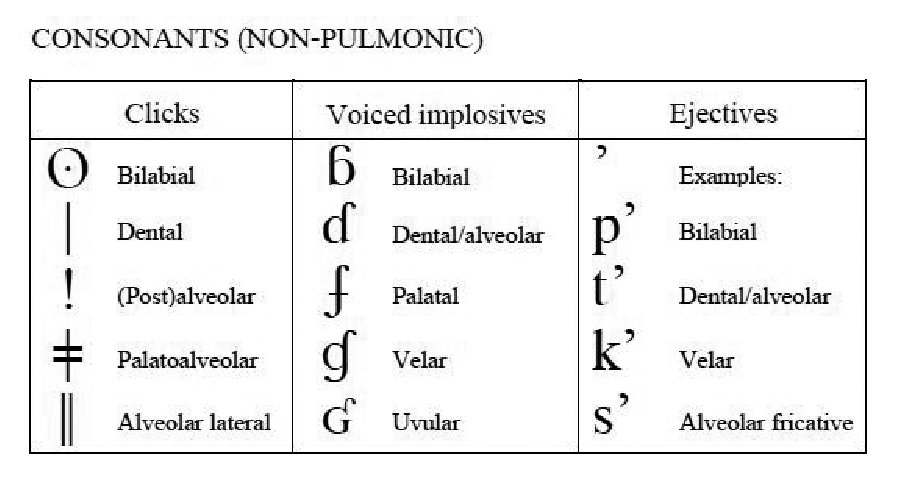
\includegraphics[scale=0.45]{material/04ipaconsonantnonpulmonic}
%		\caption{Konsonanten (Nicht Pulmonal)}
%		%\label{Zeichen1}
%	\end{figure}
	
	\begin{itemize}
		\item \textbf{VIDEO:} \href{run:material/04namaclicks.mp4}{!Nama Clicks}
	\end{itemize}
			
\end{frame}



%%%%%%%%%%%%%%%%%%%%%%%%%%%%%%%%%%%%%%%%%%%%%%%%%%%%%%%%%%%%%%%%%%%

\begin{frame}
\frametitle{Vokale im IPA-Alphabet: Das Vokalviereck}

%	\begin{figure}[H]
%		\centering
%		
%		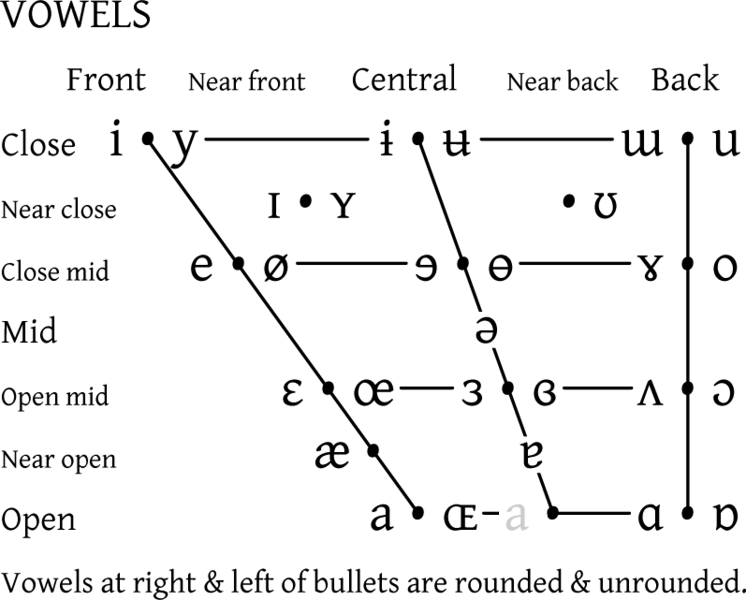
\includegraphics[scale=0.27]{material/04ipavowelwikicommons}
%		\caption{Vokale}
%		%old picture
%		%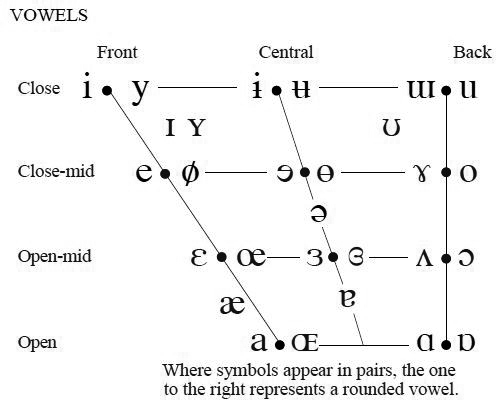
\includegraphics[scale=0.45]{material/04ipavowel}
%		%\caption{Vokale}
%		%\label{Zeichen1}
%	\end{figure}


\centerline{
	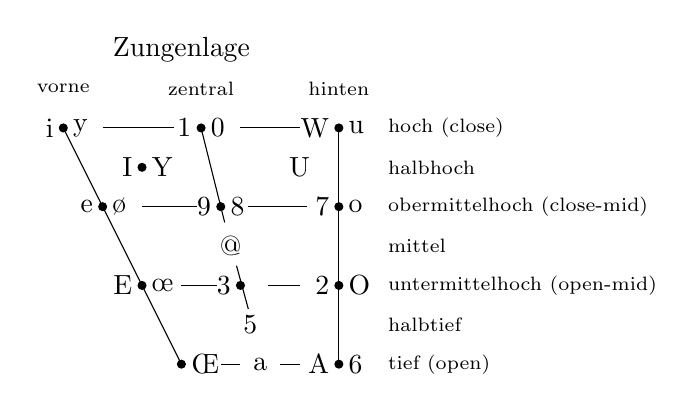
\begin{tikzpicture}
	\draw[fill] (0,0) circle [radius=0.05];
	\draw[fill] (-0.5,1) circle [radius=0.05];
	\draw[fill] (-1,2) circle [radius=0.05];
	\draw[fill] (-1.5,3) circle [radius=0.05];
	\draw[black] (0.5,0)--(0.75,0);
	\draw[black] (1.25,0)--(1.5,0);
	\draw[fill] (2,0) circle [radius=0.05];
	\draw[fill] (2,1) circle [radius=0.05];
	\draw[fill] (2,2) circle [radius=0.05];
	\draw[fill] (2,3) circle [radius=0.05];
	\draw[fill] (0.25,3) circle [radius=0.05];
	\draw[black] (0.25,3)--(0.55,1.8);
	\draw[black] (-0.1,3)--(-1,3);
	\draw[black] (0.75,3)--(1.5,3);
	\draw[fill] (0.5,2) circle [radius=0.05];
	\draw[fill] (0.75,1) circle [radius=0.05];
	\draw[black](0.7,1.25)--(0.85,0.7);
	\node[right] at (0.25,3){\textipa{0}};
	\node[left] at (0.25,3){\textipa{1}};
	\node at (0,4){Zungenlage};
	\node at (-1.5,3.5){{\scriptsize vorne}};
	\node at (0.25,3.5){\scriptsize zentral};
	\node at (2,3.5){{\scriptsize hinten}};
	\node[right] at (2.5,3){\scriptsize hoch (close)};
	\node[right] at (2.5,2.5){\scriptsize halbhoch};
	\node[right] at (2.5,2){\scriptsize obermittelhoch (close-mid)};
	\node[right] at (2.5,1.5){\scriptsize mittel};
	\node[right] at (2.5,1){\scriptsize untermittelhoch (open-mid)};
	\node[right] at (2.5,0.5){\scriptsize halbtief};
	\node[right] at (2.5,0){\scriptsize tief (open)};
	\node[left] at (2,3){\textipa{W}};
	\node[right] at (2,3){\textipa{u}};
	\node at (1.5,2.5){\textipa{U}};
	\node[left] at (2,2){\textipa{7}};
	\node[right] at (2,2){\textipa{o}};
	\node[left] at (2,1){\textipa{2}};
	\node[right] at (2,1){\textipa{O}};
	\node[right] at (2,0){\textipa{6}};
	\node[left] at (2,0){\textipa{A}};
	\draw[black] (2,0)--(2,3);
	\node[left] at (0.5,2){\textipa{9}};
	\node[right] at (0.5,2){\textipa{8}};
	\node at (0.625,1.5){\textipa{@}};
	\node[left] at (0.75,1){\textipa{3}};
	\node[right] at (0.75,1){\textipa{\textcloserevepsilon}};
	\node at (0.875,0.5){\textipa{5}};
	\node at (1,0){\textipa{a}};
	\node[right] at (-1.5,3){\textipa{y}};
	\node[left] at (-1.5,3){\textipa{i}};
	\node[left] at (-0.5,2.5){\textipa{I}};
	\node[right] at (-0.5,2.5){\textipa{Y}};
	\draw[fill] (-0.5,2.5) circle [radius=0.05];
	\node[right] at (-1,2){\textipa{\o}};
	\node[left] at (-1,2){\textipa{e}};
	\node[right] at (-0.5,1){\textipa{\oe}};
	\node[left] at (-0.5,1){\textipa{E}};
	\node[right] at (0,0){\textipa{\OE}};
	\draw[black] (0,0)--(-1.5,3);
	\draw[black] (-0.5,2)--(0.2,2);
	\draw[black] (0.85,2)--(1.6,2);
	\draw[black] (0,1)--(0.45,1);
	\draw[black] (1.1,1)--(1.5,1);
	\end{tikzpicture}
}
        
        Vokale links des Punktes sind ungerundet,\\
        die rechts sind gerundet.

%=======
%	\begin{figure}[H]
%		\centering
%		
%		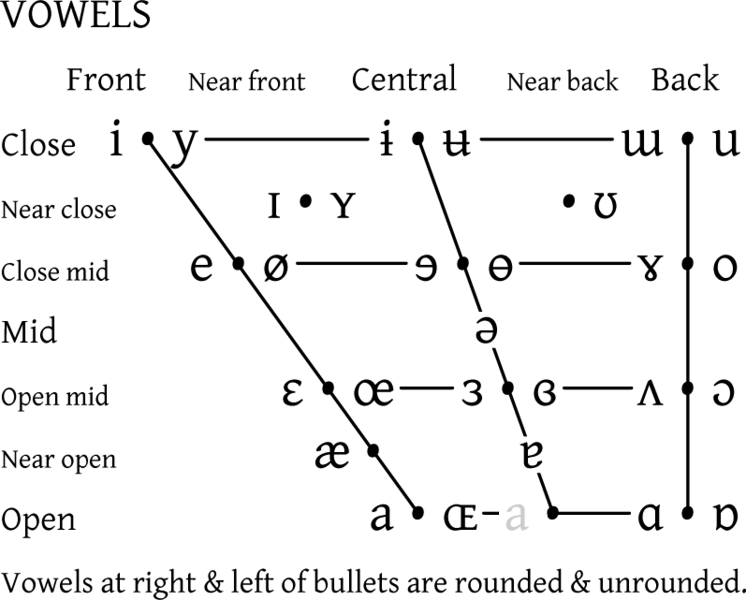
\includegraphics[scale=0.27]{material/04ipavowelwikicommons}
%%		\caption{Vokale}
%		%old picture
%		%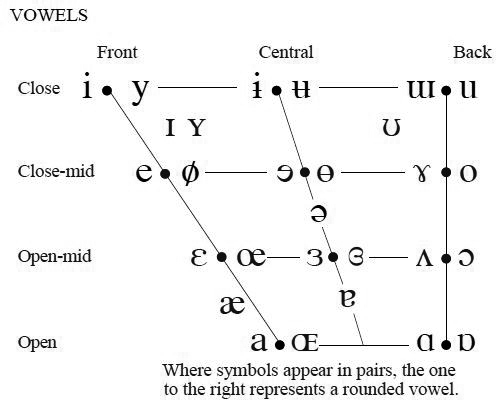
\includegraphics[scale=0.45]{material/04ipavowel}
%		%\caption{Vokale}
%		%\label{Zeichen1}
%	\end{figure}
	
\end{frame}


%% %%%%%%%%%%%%%%%%%%%%%%%%%%%%%%%%%
\begin{frame}
\frametitle{Vokale im Deutschen}

\noindent
\begin{minipage}{.55\textwidth}
	\centerline{
	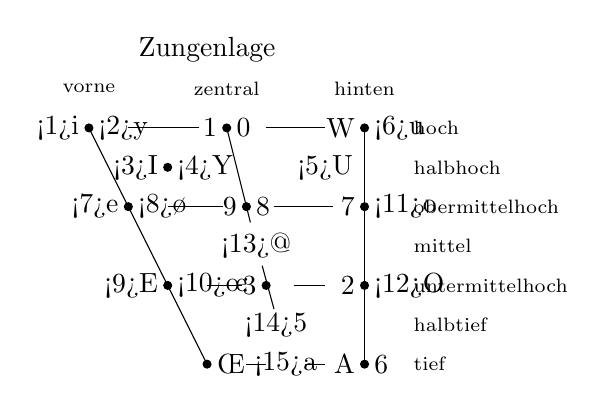
\begin{tikzpicture}
	\draw[fill] (0,0) circle [radius=0.05];
	\draw[fill] (-0.5,1) circle [radius=0.05];
	\draw[fill] (-1,2) circle [radius=0.05];
	\draw[fill] (-1.5,3) circle [radius=0.05];
	\draw[black] (0.5,0)--(0.75,0);
	\draw[black] (1.25,0)--(1.5,0);
	\draw[fill] (2,0) circle [radius=0.05];
	\draw[fill] (2,1) circle [radius=0.05];
	\draw[fill] (2,2) circle [radius=0.05];
	\draw[fill] (2,3) circle [radius=0.05];
	\draw[fill] (0.25,3) circle [radius=0.05];
	\draw[black] (0.25,3)--(0.55,1.8);
	\draw[black] (-0.1,3)--(-1,3);
	\draw[black] (0.75,3)--(1.5,3);
	\draw[fill] (0.5,2) circle [radius=0.05];
	\draw[fill] (0.75,1) circle [radius=0.05];
	\draw[black](0.7,1.25)--(0.85,0.7);
	\node[right] at (0.25,3){\textipa{0}};
	\node[left] at (0.25,3){\textipa{1}};
	\node at (0,4){Zungenlage};
	\node at (-1.5,3.5){{\scriptsize vorne}};
	\node at (0.25,3.5){\scriptsize zentral};
	\node at (2,3.5){{\scriptsize hinten}};
	\node[right] at (2.5,3){\scriptsize hoch};
	\node[right] at (2.5,2.5){\scriptsize halbhoch};
	\node[right] at (2.5,2){\scriptsize obermittelhoch};
	\node[right] at (2.5,1.5){\scriptsize mittel};
	\node[right] at (2.5,1){\scriptsize untermittelhoch};
	\node[right] at (2.5,0.5){\scriptsize halbtief};
	\node[right] at (2.5,0){\scriptsize tief};
	\node[left] at (2,3){\textipa{W}};
	\node[right] at (2,3){\rotul{\gruen<6>{\textipa{u}}}};
	\node at (1.5,2.5){\rotul{\gruen<5>{\textipa{U}}}};
	\node[left] at (2,2){\textipa{7}};
	\node[right] at (2,2){\rotul{\gruen<11>{\textipa{o}}}};
	\node[left] at (2,1){\textipa{2}};
	\node[right] at (2,1){\rotul{\gruen<12>{\textipa{O}}}};
	\node[right] at (2,0){\textipa{6}};
	\node[left] at (2,0){\textipa{A}};
	\draw[black] (2,0)--(2,3);
	\node[left] at (0.5,2){\textipa{9}};
	\node[right] at (0.5,2){\textipa{8}};
	\node at (0.625,1.5){\rotul{\gruen<13>{\textipa{@}}}};
	\node[left] at (0.75,1){\textipa{3}};
	\node[right] at (0.75,1){\textipa{\textcloserevepsilon}};
	\node at (0.875,0.5){\rotul{\gruen<14>{\textipa{5}}}};
	\node at (1,0){\rotul{\gruen<15>{\textipa{a}}}};
	\node[right] at (-1.5,3){\rotul{\gruen<2>{\textipa{y}}}};
	\node[left] at (-1.5,3){\rotul{\gruen<1>{\textipa{i}}}};
	\node[left] at (-0.5,2.5){\rotul{\gruen<3>{\textipa{I}}}};
	\node[right] at (-0.5,2.5){\rotul{\gruen<4>{\textipa{Y}}}};
	\draw[fill] (-0.5,2.5) circle [radius=0.05];
	\node[right] at (-1,2){\rotul{\gruen<8>{\textipa{\o}}}};
	\node[left] at (-1,2){\rotul{\gruen<7>{\textipa{e}}}};
	\node[right] at (-0.5,1){\rotul{\gruen<10>{\textipa{\oe}}}};
	\node[left] at (-0.5,1){\rotul{\gruen<9>{\textipa{E}}}};
	\node[right] at (0,0){\textipa{\OE}};
	\draw[black] (0,0)--(-1.5,3);
	\draw[black] (-0.5,2)--(0.2,2);
	\draw[black] (0.85,2)--(1.6,2);
	\draw[black] (0,1)--(0.45,1);
	\draw[black] (1.1,1)--(1.5,1);
	\end{tikzpicture}
}

\medskip

Deutsche Vokale sind \alt<handout>{unterstrichen}{rot}
\end{minipage}
\hfill
\begin{minipage}{.42\textwidth}
	\begin{itemize}
	\item Liege [\textipa{li:g@}]\pause,  Lüge [\textipa{ly:g@}]\pause
	\item Kiste [\textipa{kIst@}]\pause,  Küste [\textipa{kYst@}]\pause
	\item muss [\textipa{mUs}]\pause,   Mus   [\textipa{mu:s}]\pause
	\item Wege  [\textipa{ve:g@}]\pause,  wöge [\textipa{vø:g@}]\pause
	\item helle [\textipa{hEl@}]\pause,   Hölle [\textipa{hœl@}]\pause
	\item Ofen  [\textipa{o:f@n}]\pause,  offen [\textipa{Of@n}]\pause
	\item geben [\textipa{ge:b@n}]\pause, Lehrer [\textipa{le:K5}]\pause
	\item Lab   [\textipa{la:p}]
	\end{itemize}
\end{minipage}
\end{frame}
%%%%%%%%%%%%%%%%%%%%%%%%%%%%%%%


\begin{frame}
\frametitle{Suprasegmentalia}

\begin{tabular}{l|p{6cm}|p{3cm}}
	\textbf{Zeichen} 		&	\textbf{Erklärung}				& \textbf{Beispiel} \\
	\hline
\textipa{\textprimstress} & Hauptbetonung 				&[\textipa{apo\textprimstress te:k@}]\\
\textipa{\textsecstress} 	&Nebenbetonung 	& [\textipa{\textprimstress ba:nho:fs\textsecstress hal@}]\\
\textipa{:} 						& lang 										& [\textipa{ba:n}] (vs. [\textipa{ban}])\\
\textipa{;} 						&	halblang 											& \\
\textipa{\u{}} 					&extra-kurz/ unsilbischer Vokal 			& [\textipa{stu:d\u{i}@}] \\
\textipa{\textvertline} 			&untergeordnete Intonationsgruppe &\\
 \textipa{\textdoublevertline} &	übergeordnete Intonationsgruppe		&	\\
  \textipa{.} 						&		Silbengrenze							&[\textipa{\textprimstress zIl.bEn.\textsecstress gKEn.\t{ts}@}]\\
  \textipa{\t{}} &				Doppelartikulation& [\textipa{P\t{aU}to:}],  [\textipa{nE\t{ts}}] \\
\end{tabular}

%	\item 
%	\item 
%	\item 
%	\item
%	\item
%	\item  	
	\end{frame}


%%%%%%%%%%%%%%%%%%%%%%%%%%%%%%%%%%%%%%%%%%%%%%%%%%%%%%%%%%%%%%%%
%%%%%%%%%%%%%%%%%%%%%%%%%%%%%%%%%%%%%%%%%%%%%%%%%%%%%%%%%%%%%%%%
%
\subsection{Artikulatorische Phonetik}
\iftoggle{toc}{
\frame{
\begin{multicols}{2}
	\tableofcontents[currentsection]
\end{multicols}
}
}
\outline{

\begin{itemize}

\item Einführung
\item Bereiche der Phonetik
\item  Methodik
\item  Probleme der Phonetik
\item  IPA-Alphabet
\item \blaubf{Artikulatorische Phonetik}
  \begin{itemize}
\item Konsonanten
\item Konsonantenklassiffikation
\item Vokale
  \item Vokalklassiffikation
\item Vokalviereck
\item Monophthong, Diphthong, Triphthong
    \end{itemize}
\item Übungen
  
  \end{itemize}
}

%%%%%%%%%%%%%%%%%%%%%%%%%%%%%%%%%%%%%%%%%%%%%%%%%%%%%%%%%%%%%%%%

\begin{frame}{Artikulatorische Phonetik: Initiator, Generator, Modifikator}

Mehrere Körperteile sind für Erzeugung von Schall nötig:
		
		\begin{itemize}
			\item \textbf{Initiator}: die Lunge \ras (Atmung) erzeugt Luftstrom
			\item \textbf{Generator}: der Kehlkopf (Larynx) mit den Stimmbändern \ras\\
                              Luftstrom wird in Schwingung versetzt (Phonation)

			\item[] Frequenz: Häufigkeit mit der die Stimmlippen schwingen bestimmt die Tonhöhe:
			        Bei Frauen ung. 230 Hz, bei Männern 120 Hz und bei Säuglingen 400 Hz
			

			\item[] \textbf{VIDEO:} \href{run:material/04TransNasalEndoscopy.mp4}{Trans-Nasal Endoscopy}

		        \item \textbf{Modifikator}: Rachen-, Mund- und Nasenraum mit den verschiedenen
                  Sprechwerkzeugen (Zunge, Lippen, weicher Gaumen) \ras\\
                  Unterschiedliche Stellung der Artikulationsorgane verändert den Rohschall des Kehlkopfs zu den wohlunterschiedenen Lauten (Artikulation im engeren Sinne).
	\end{itemize}

                
	
\end{frame}


%%%%%%%%%%%%%%%%%%%%%%%%%%%%%%%%%%%%%%%%%%%%%%%%%%%%%%%%%%%%%%%%

%% \begin{frame}
%% \frametitle{Artikulatorische Phonetik: Modifikator}

%% 	\begin{itemize}
%% 		\item \textbf{Modifikator}: Rachen-, Mund- und Nasenraum mit den verschiedenen
%%                   Sprechwerkzeugen (Zunge, Lippen, weicher Gaumen) \ras\\
%%                   Unterschiedliche Stellung der Artikulationsorgane verändert den Rohschall des Kehlkopfs zu den wohlunterschiedenen Lauten (Artikulation im engeren Sinne).
%% 	\end{itemize}
	
%% \end{frame}



%%%%%%%%%%%%%%%%%%%%%%%%%%%%%%%%%%%%%%%%%%%%%%%%%%%%%%%%%%%%%%%%%%%%%%%%%%%%%%%%%%%%%%%%%%%%%%%%%%%%%%%%%%%%%%%%%%%%%%%%%%%%%%%%
%
\subsubsection{Konsonanten}
%\frame{
%\begin{multicols}{2}
%	\tableofcontents[currentsection]
%\end{multicols}
%}
%%%%%%%%%%%%%%%%%%%%%%%%%%%%%%%%%%%%%%%%%%%%%%%%%%%%%%%%%%%%%%%%

\begin{frame}{Konsonanten}

	\begin{itemize}
		\item Konsonanten \ras Mitlaute
		\item[]
		\item Die Artikulationsorgane bilden eine \textbf{geräuschverursachende Enge} oder einen Verschluss im Ansatzrohr, d.\,h. die Luft wird oberhalb der Stimmritze (Glottis) zwischen den Stimmbändern behindert.
	\end{itemize}
	
\end{frame}


%%%%%%%%%%%%%%%%%%%%%%%%%%%%%%%%%%%%%%%%%%%%%%%%%%%%%%%%%%%%%%%%

\begin{frame}
\frametitle{Sagittalschnitt}

\begin{minipage}{0.48\textwidth}
	\begin{figure}
	\centering
	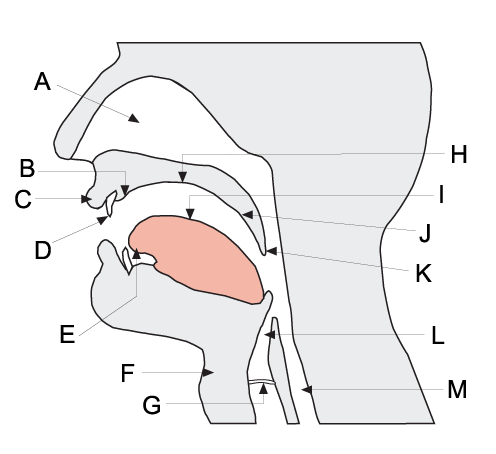
\includegraphics[scale=0.32]{material/04phonoatonomy}
	\caption{Sagittalschnitt, CC BY-SA 3.0}
	\end{figure}
\end{minipage}\hfill
\begin{minipage}{0.4\textwidth}
	A -- Nasenraum\\
	B -- Zahndamm \emph{Alveolen}\\
	C -- (Ober)Lippe \\
	D -- (obere) Zähne\\
	E -- Zugenspitze \emph{Apex}\\
	F -- Kehlkopf \emph{Larynx}\\
	G -- Stimmlippen \emph{Glottis}\\
	H -- harter Gaumen \emph{Palatum}\\
	I -- Zungenrücken \emph{Dorsum}\\
	J -- Gaumensegel \emph{Velum}\\
	K -- Zäpfchen \emph{Uvula}\\
	L -- Luftröhre\\ 
	M -- Speiseröhre
\end{minipage}
	
%	\begin{figure}[H] %%altes Bild%%
%		\centering
%		
%		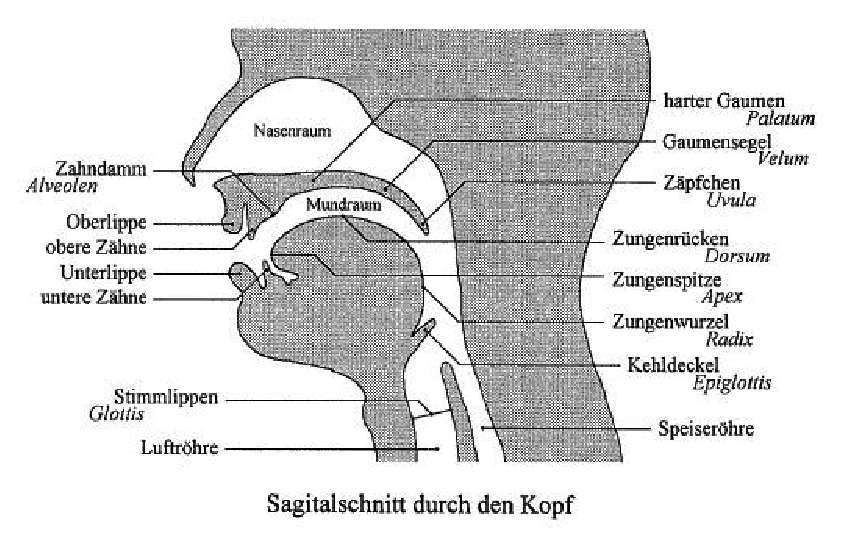
\includegraphics[scale=0.65]{material/04sagitalschnittaltmann}
%		\caption{Sagitalschnitt \citep{Altmann&Co07a}}
%		%\label{Zeichen1}
%	\end{figure}
	
\end{frame}



%%%%%%%%%%%%%%%%%%%%%%%%%%%%%%%%%%%%%%%%%%%%%%%%%%%%%%%%%%%%%%%%
%%%%%%%%%%%%%%%%%%%%%%%%%%%%%%%%%%%%%%%%%%%%%%%%%%%%%%%%%%%%%%%%
%
\subsubsection{Konsonantenklassifikation}
%
%%%%%%%%%%%%%%%%%%%%%%%%%%%%%%%%%%%%%%%%%%%%%%%%%%%%%%%%%%%%%%%%

\begin{frame}{Konsonantenklassifikation: Stimmbeteiligung}

	\begin{itemize}
		\item \textbf{Stimmbeteiligung} (Stimmhaftigkeit): Schwingungszustand der Stimmbänder
		
		\begin{itemize}
			\item[]
			\item \textbf{stimmhaft} \ras eng beieinander stehende Stimmbänder
			\item[]
			\item \textbf{stimmlos} \ras weit auseinander stehende Stimmbänder

			\ea \textipa{[ p ]} vs. \textipa{[ b ]}
			\z

			\item[]
			\item \textbf{Aspiration} (Behauchung): Glottis während der Verschlussphase ist weit gespreizt und schwingt mit.

			\ea \textipa{[ \super h ]}
			\z

                        \textbf{VIDEO:} \href{run:material/02-aspiration.mp4}{Aspiration}
		\end{itemize}

	\end{itemize}
	
\end{frame}



%%%%%%%%%%%%%%%%%%%%%%%%%%%%%%%%%%%%%%%%%%%%%%%%%%%%%%%%%%%%%%%%

\begin{frame}
\frametitle{Übung}

Welche der folgenden Laute sind stimmhaft und welche stimmlos?

		\ea \textipa{[ d, z, f, v, g, k, P ]}
		\z

		\pause
Lösung:
\begin{itemize}
\item stimmhaft: \textipa{[ d, z, v, g ]}
\item stimmlos: \textipa{[ f, k, P ]}
\end{itemize}
\end{frame}

%%%%%%%%%%%%%%%%%%%%%%%%%%%%%%%%%%%%%%%%%%%%%%%%%%%%%%%%%%%%%%%%

\begin{frame}
\frametitle{Konsonantenklassifikation: Stellung des Gaumensegels}

	\begin{itemize}
		\item \textbf{Stellung des Gaumensegels} (des weichen Gaumens):
		
		\begin{itemize}
			\item[]
			\item Nasale Laute (\zB \textipa{ [ m , n ]}) \ras Senkung des weichen Gaumens (Velum)
			\item[]
			\item Orale Laute (\zB \textipa{ [ f , a ]}) \ras bei gehobenem Velum
		\end{itemize}
		
		\item[]
		\item \textbf{LINK:} Interaktiver Sagittalschnitt: \url{http://smu-facweb.smu.ca/~s0949176/sammy/}
	\end{itemize}
	
\end{frame}


%%%%%%%%%%%%%%%%%%%%%%%%%%%%%%%%%%%%%%%%%%%%%%%%%%%%%%%%%%%%%%%%

\begin{frame}
\frametitle{Konsonantenklassifikation: Artikulationsort}

	\begin{itemize}
	\item \textbf{Artikulationsort} im Vokaltrakt: Ort, an dem die Luft behindert wird.
          Unterscheidung nach nicht-beweglichen und beweglichen Artikulatoren.

		\item[]
		\item \textbf{Nicht-bewegliche} Artikulatoren (passiver Artikulator, Artikulationsort im engeren Sinne):
			
		\begin{itemize}
			\item die oberen Zähne \ras \textbf{dental}
			\item[]
			\item die Alveolen (Knochendamm hinter den oberen Zähne) \ras \textbf{alveolar}
			\item[]
			\item der harte Gaumen (Palatum) \ras \textbf{palatal}
		\end{itemize}
		
	\end{itemize}
	
\end{frame}


%%%%%%%%%%%%%%%%%%%%%%%%%%%%%%%%%%%%%%%%%%%%%%%%%%%%%%%%%%%%%%%%

\begin{frame}
\frametitle{Konsonantenklassifikation: Artikulationsort II}

\begin{itemize}
	\item \textbf{Bewegliche} Artikulatoren (aktiver Artikulator, Artikulationsorgan):
			
	\begin{itemize}
		\item[]
		\item weicher Gaumen (Velum) \ras \textbf{velar}
		\item[]
		\item das Zäpfchen (Uvula) \ras \textbf{uvular}
		\item[]
		\item Lippen \ras \textbf{labial}
		\item[]
		\item Unterkiefer
		\item[]
		\item Zunge
	\end{itemize}

\end{itemize}

\end{frame}


%%%%%%%%%%%%%%%%%%%%%%%%%%%%%%%%%%%%%%%%%%%%%%%%%%%%%%%%%%%%%%

\begin{frame}
\frametitle{Konsonantenklassifikation: Weitere Unterteilung}

		\begin{itemize}
			\item[]
			\item Bei der Artikulation mit der Zunge bildet man Untergruppen nach dem beteiligten Zungenteil:
			
			\begin{itemize}
				\item[]
				\item \textbf{koronal}: mit dem vorderen Teil der Zunge\\
				\ras \textbf{apikal}: mit der Zungenspitze\\
				\ras \textbf{laminal}: mit dem Zungenblatt (mittlerer Teil der Zunge)

				\ea \textipa{[ t, d, l, n, s, z, S, Z ]}
				\z

				\item \textbf{dorsal}: mit dem hinteren Teil der Zunge

				\ea \textipa{[ \c{c}, j, g, k, x, N, \textscr , K ]}
				\z

			\end{itemize}

					\item[]
		\item \textbf{LINK:} Interaktiver Sagittalschnitt: \url{http://smu-facweb.smu.ca/~s0949176/sammy/}

		\end{itemize}
		

	
\end{frame}


%%%%%%%%%%%%%%%%%%%%%%%%%%%%%%%%%%%%%%%%%%%%%%%%%%%%%%%%%%%%%%%%

\begin{frame}
\frametitle{Konsonantenklassifikation: Artikulationsart}

	\begin{itemize}
	\item \textbf{Artikulationsart} (Artikulationsmodus):\\
               Art der Behinderung des Luftstroms durch die Artikulationsorgane

			\item[]
			\item \textbf{Plosive} (Verschlusslaute, Explosivlaute, stops): totaler oraler Verschluss mit anschließender plötzlicher Lösung des Verschlusses\\
	Das Velum bleibt dabei in angehobener Position, so dass die Luft durch den Mundraum strömt.

			\ea \textipa{[ p, b, t, d, k, g, P ]}
			\z
			
			Der \textbf{Glottalverschluss} (Knacklaut) \textipa{[ P ]} entsteht durch plötzliches Öffnen der Stimmritze und kommt im Deutschen vor anlautendem Vokal eines Wortes und vor anlautendem Vokal in einer betonten Silbe vor.
		
	\end{itemize}
	
\end{frame}


%%%%%%%%%%%%%%%%%%%%%%%%%%%%%%%%%%%%%%%%%%%%%%%%%%%%%%%%%%%%%%%%

\begin{frame}
\frametitle{Artikulationsart: Frikative}

		\begin{itemize}
			\item \textbf{Frikative} (Reibelaute, Spiranten): Verengung zweier Sprechorgane,\\
                          Luftstrom strömt durch die Verengung, es entsteht ein Reibegeräusch.

			\ea \textipa{[ f, v, s, z, S, Z, \c{c}, x, h, K ]}
			\z
			
			\begin{itemize}
				\item \textbf{Sibilanten} (Zischlaut): Unterklasse der Frikative mit intensivem, hochfrequentem Geräuschanteil.

				\ea \textipa{[ s, z, S ]}
				\z

		\end{itemize}
		
	\end{itemize}
	
\end{frame}


%%%%%%%%%%%%%%%%%%%%%%%%%%%%%%%%%%%%%%%%%%%%%%%%%%%%%%%%%%%%%%%%

\begin{frame}
%\frametitle{Konsonantenklassifikation}
\frametitle{Artikulationsart: Affrikaten}

		\begin{itemize}
			\item \textbf{Affrikaten}: Plosive, die in Frikative übergehen, wobei die Verschlussphase und die Frikativphase dieselbe (oder annähernd dieselbe) Artikulationsstelle haben; d.\,h. sie sind \textbf{homorgan}.

			\ea \textipa{[ \t{pf} , \t{ts} , \t{tS} , \t{dZ} ]}
			\z

			\begin{itemize}
				\item Per Definitionem gehören der plosive und der frikative Laut einer Affrikaten \textbf{zum selben Morphem} (die kleinste bedeutungstragende Einheit). Daraus ergibt sich:

				\ea \textipa{[ \t{ts} ]} in \ab{Blitz} \ras Affrikate
				\z
				
				\ea \textipa{[ ts ]} in \ab{Monats} \ras keine Affrikate
				\z

			\end{itemize}
		
		\item[]
		\item Plosive, Frikative und Affrikaten \ras \textbf{Obstruenten}
	\end{itemize}
	
\end{frame}


%%%%%%%%%%%%%%%%%%%%%%%%%%%%%%%%%%%%%%%%%%%%%%%%%%%%%%%%%%%%%%%%

\begin{frame}
\frametitle{Artikulationsart: Vibranten}

		\begin{itemize}
			\item \textbf{Vibranten} (trills): schnelle Folge oraler Verschlüsse
			\begin{itemize}
				\item[]
				\item Artikulationsstellen für Vibranten sehr eingeschränkt: nur bilabial, alveolar oder uvular
				\item[]
				\item Der alveolare Vibrant \textipa{[ r ]} (das sog. Zungenspitzen-R) kommt in vielen süddeutschen Varietäten vor.
				\item[]
				\item Der uvulare Vibrant \textipa{[ \textscr\ ]} (das gerollte Zäpfchen-R) ist eine häufige Realisierung des Deutschen \ab{r}.
			\end{itemize}
			 
	\end{itemize}
	
\end{frame}


%%%%%%%%%%%%%%%%%%%%%%%%%%%%%%%%%%%%%%%%%%%%%%%%%%%%%%%%%%%%%%%%

\begin{frame}
\frametitle{Artikulationsart: Approximanten}

		\begin{itemize}
			\item \textbf{Approximanten} (Öffnungslaute): Enge im Ansatzrohr (wie Frikative)\\
			Bei Approximanten gibt es nicht so eine große Nähe zwischen Artikulator und Artikulationsstelle \ras kein Reibegeräusch
			\item[]
			\item[] Zwei Unterklassen:
			
			\begin{itemize}
				\item[]
				\item \textbf{Laterale}: Verschluss in der Mundhöhlenmitte, Luft entweicht seitlich [~\textipa{l}~]
				\item[]
				\item \textbf{Gleitlaute} (zentral): zentrale Verengung aber weiter als bei Frikativen [~\textipa{w}~].\\
				(Manchmal wird [~\textipa{j}~] auch zu den Gleitlauten gezählt,\\
                                  da die Verengung weiter als bei anderen Frikativen ist. Dies ist jedoch strittig!)
			\end{itemize}
			
		\end{itemize}	

\end{frame}


%%%%%%%%%%%%%%%%%%%%%%%%%%%%%%%%%%%%%%%%%%%%%%%%%%%%%%%%%%%%%%%%

\begin{frame}
%\frametitle{Konsonantenklassifikation}
\frametitle{Artikulationsart: Nasale}
		\begin{itemize}
			\item \textbf{Nasale}: totaler oraler Verschluss (wie Plosive). Luft entweicht durch die Nase durch Senken des Velums\\
			\item[] Im Deutschen kommen 3 Nasale vor: \textipa{[ m, n, N ]}

		\item[]
		\item Vibranten, Approximanten (Laterale und Gleitlaute), Nasale und Vokale (auch die hier nicht behandelten \gqq{geschlagenen Laute} wie das span. \textipa{[~R~]}) gehören zur Gruppe der \textbf{Sonoranten}, da die Luft bei denen ungehindert ausströmen kann. Sonoranten sind \textbf{immer} stimmhaft!
		\item[]
		\item Die Klasse der l-Laute und r-Laute werden auch zu den sog. \textbf{Liquiden} zusammengefasst (im Dt. \textipa{[ l, r, \textscr ]})
	\end{itemize}
	
\end{frame}


%%%%%%%%%%%%%%%%%%%%%%%%%%%%%%%%%%%%%%%%%%%%%%%%%%%%%%%%%%%%%%%%

\begin{frame}
\frametitle{Konsonantenklassifikation: Zusammenfassung}

	\begin{itemize}
		\item Für die \textbf{Differenzierung der deutschen Konsonanten} sind hauptsächlich 3 Merkmale wichtig:
		
		\begin{itemize}
			\item[]
			\item Stimmbeteiligung
			\item Artikulationsort
			\item Artikulationsart
		\end{itemize}
	\end{itemize}

\end{frame}

%%%%%%%%%%%%%%%%%%%%%%%%%%%%%%%%%%%%%%%%%%%%%%%%%%

\begin{frame}

  \frametitle{Übung}

\begin{itemize}
	\item [] Beschreiben Sie die Konsonanten in den folgenden Wörtern und geben Sie die entsprechenden phonetischen Symbole an:

		 	\begin{enumerate}
		 		\item Busch
		 		\item malen
		 		\item Maus
		 		\item Achtung
		 		\item Genie
		 		\item zirpen
		 		\item wichtig
		 		\item Wald
		 	\end{enumerate}

\end{itemize}
\end{frame}

%%%%%%%%%%%%%%%%%%%%%%%%%%%%%%%%%%%%%%%%%%%%%%%%%%%

\begin{frame}
\frametitle{Lösung}

\begin{table}
	\scalebox{.9}{
		\begin{tabular}{llp{9cm}}
1. Busch &{[\textipa{bUS}]} 								& b: bilabialer, stimmhafter Plosiv \textipa{S}:~postalveolarer, stimmloser Frikativ\\
\pause
2. malen & {[\textipa{\textprimstress ma:l@n}]} 	& m:~bilabialer, stimmhafter Nasal; n:~alveolarer, stimmhafter Nasal, l:~alveolaer, stimmhafter Lateral\\
\pause
3. Maus & {[\textipa{m\t{aU}s}]}							& m:~s.o.; s:~stimmloser, alveolarer Frikativ \\
\pause
4. Achtung &{[\textipa{\textprimstress aXtU\ng}]} & \textipa{X}:~velarer, stimmloser Frikativ; t:~alveolarer, stimmloser Plosiv \textipa{\ng}: velarer, stimmhafter Nasal\\
\pause
5. Genie	&{[\textipa{Ze:\textprimstress ni:}]}		& \textipa{Z}: postalveolarer, stimmhafter Frikativ, n:~s.o.\\
\pause
6. zirpen & {[\textipa{\t{ts}IKp@n}]}						& \textipa{\t{ts}}: alveolare, stimmlose Affrikate; \textipa{K}:~uvularer, stimmhafter Frikativ; p:~bilabialer, stimmloser Plosiv; n: s.o.\\
\pause
7. wichtig & {[\textipa{\textprimstress vI\c{c}tI\c{c}}]} & \textipa{v}: labiodentaler, stimmhafter Frikativ; \textipa{\c{c}}: palataler, stimmloser Frikativ t: s.o.\\
\pause
8. Wald 	&	{[\textipa{valt}]}									& v, l, t: s.o.\\
\end{tabular}}
\end{table}

\end{frame}


%%%%%%%%%%%%%%%%%%%%%%%%%%%%%%%%%%%%%%%%%%%%%%%%%%%%%%%%%%%%%%%%
%
\subsubsection{Vokale}
\iftoggle{toc}{
\frame{
\begin{multicols}{2}
	\tableofcontents[currentsection]
\end{multicols}
}
}
%%%%%%%%%%%%%%%%%%%%%%%%%%%%%%%%%%%%%%%%%%%%%%%%%%%%%%%%%%%%%%%%

\begin{frame}{Vokale}

	\begin{itemize}
		\item \textbf{Vokale} (Selbstlaute) sind Laute, bei deren Artikulation die Luft ungehindert durch den Mundraum strömen kann (deswegen gehören sie zu den Sonoranten)
		\item[]
		\item Vokale sind \idR immer stimmhaft.
		\item[]
		\item Es ist umstritten, ob der sog. Schwa-Laut im Dt. \textipa{[ @ ]} stimmhaft
                  ist.\\
                  Auch im Japanischen soll es stimmlose Vokale geben.
	\end{itemize}
	
\end{frame}


%%%%%%%%%%%%%%%%%%%%%%%%%%%%%%%%%%%%%%%%%%%%%%%%%%%%%%%%%%%%%%%%
%%%%%%%%%%%%%%%%%%%%%%%%%%%%%%%%%%%%%%%%%%%%%%%%%%%%%%%%%%%%%%%%
%
\subsubsection{Vokalklassifikation}
%
%%%%%%%%%%%%%%%%%%%%%%%%%%%%%%%%%%%%%%%%%%%%%%%%%%%%%%%%%%%%%%%%

\begin{frame}{Vokalklassifikation}

	\begin{itemize}
		\item \textbf{Zungenhöhe} (Vokalhöhe): Grad der Zungenhebung in Richtung Gaumen

		\ea hoch: \textipa{[ i: ]}, mittel: \textipa{[ o: ]}, tief: \textipa{[ a: ]} bzw. geschlossen, halboffen, offen
		\z

		\item \textbf{Zungenlage} (Vokaltiefe): angehobener Teil der Zunge

		\ea vorne: \textipa{[ i: ]}, zentral: \textipa{[ a: ]}, hinten: \textipa{[ u: ]}
		\z

		\item \textbf{Lippenrundung}: Art der Lippenöffnung

		\ea gerundet: \textipa{[ o: ]}, ungerundet: \textipa{[ i: ]}
		\z

		\bigskip
                
		\item\textbf{ÜB:} Lesen Sie folgende Wörter mit gerundeten und mit gespreizten Lippen:
		\item[] Bühne, rühmen, Dünen, Stiele, Trieb, Möhre, Herd, Hefe
                  \pause
                  
                        Biene, Riemen, dienen, Stühle, trüb, Meere, hört, Höfe
	\end{itemize}
	
\end{frame}


%%%%%%%%%%%%%%%%%%%%%%%%%%%%%%%%%%%%%%%%%%%%%%%%%%%%%%%%%%%%%%%%

\begin{frame}
\frametitle{Vokalklassifikation: Gespanntheit}

	\begin{itemize}
		\item \textbf{Gespanntheit} vs. Ungespanntheit der Muskeln (Länge, Vokalquantität):
		
		\begin{itemize}
			\item[]
			\item Definition 1: \textipa{[ i:, y:, u:, o: ]} \textbf{mehr Muskelspannung} als \textipa{[ I, Y, U , O ]}\\
			(von der experimentellen Phonetik weder bestätigt noch widerlegt)
			\item[]
			\item Definition 2: mit vorverlagerter Zungenwurzel
			\item[]
			\item I.\;d.\;R. alle tiefen Vokale \ras ungespannt (strittig!)
			\item langer tiefer Vokal \textipa{[ a: ]} \ras gespannt(?)
		\end{itemize}

	      \item Im Deutschen: Korrelation der Gespanntheit mit der Länge.

		\ea \textipa{[ m i: t @ ]} vs. \textipa{[ m I t @ ]}
		\z

		\item In Lehnwörtern auch kurze gespannte Vokale

		\ea \textipa{[ P i . d e: ]}
		\z
		
	\end{itemize}
	
\end{frame}


%%%%%%%%%%%%%%%%%%%%%%%%%%%%%%%%%%%%%%%%%%%%%%%%%%%%%%%%%%%%%%%%

\begin{frame}
\frametitle{Vokalklassifikation: Stellung des Gaumensegels}

	\begin{itemize}
	
		
%\vspace{1em}
		
		\item \textbf{Stellung des Gaumensegels}:
		
		\begin{itemize}
			\item oral
			\item nasal
			\item[]
			\item Nasalvokale kommen im Dt. nur in Lehnwörtern vor.

			\eal
			\ex \textipa{[ \~a ]} in \ab{Gourm\textbf{and}}
			\ex \textipa{[ \~E ]} in \ab{T\textbf{eint}}
			\ex \textipa{[ \~a ]} in \ab{Restaur\textbf{ant}}
			\ex \textipa{[ \~\oe\ ]} in \ab{in Parf\textbf{um}}
			\zl
		
		\end{itemize}
		
	\end{itemize}
	
\end{frame}


%%%%%%%%%%%%%%%%%%%%%%%%%%%%%%%%%%%%%%%%%%%%%%%%%%%%%%%%%%%%%%%%

\begin{frame}
\frametitle{Vokalklassifikation: Überblick}

	\begin{itemize}
		\item Für die Differenzierung der deutschen nativen Vokale sind hauptsächlich vier Merkmale wichtig:
		
		\begin{itemize}
			\item[]
			\item Zungenhöhe
			\item[]
			\item Zungenlage
			\item[]
			\item Lippenrundung
			\item[]
			\item Gespanntheit (bzw. Länge)
		\end{itemize}
		
	\end{itemize}
	
\end{frame}


%%%%%%%%%%%%%%%%%%%%%%%%%%%%%%%%%%%%%%%%%%%%%%%%%%%%%%%%%%%%%%%%
%%%%%%%%%%%%%%%%%%%%%%%%%%%%%%%%%%%%%%%%%%%%%%%%%%%%%%%%%%%%%%%%
%
\subsubsection{Vokalviereck}
%\frame{
%\begin{multicols}{2}
%	\tableofcontents[currentsection]
%\end{multicols}
%}
%%%%%%%%%%%%%%%%%%%%%%%%%%%%%%%%%%%%%%%%%%%%%%%%%%%%%%%%%%%%%%%%

\begin{frame}{Vokalviereck}

	\begin{itemize}
		\item Für eine bessere Darstellung wurden die Vokale (von Daniel Jones 1920) in das sog. Vokalviereck angeordnet, welches eine stilisierte Version des Vokalraums darstellt.
	\end{itemize}

\begin{figure}
	\centering
\scalebox{.8}{	
	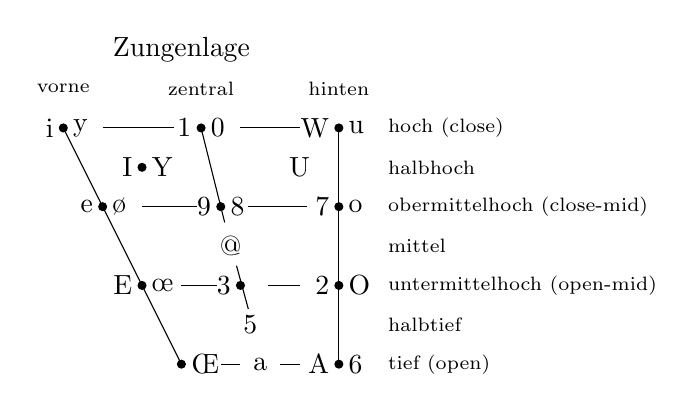
\begin{tikzpicture}
	\draw[fill] (0,0) circle [radius=0.05];
	\draw[fill] (-0.5,1) circle [radius=0.05];
	\draw[fill] (-1,2) circle [radius=0.05];
	\draw[fill] (-1.5,3) circle [radius=0.05];
	\draw[black] (0.5,0)--(0.75,0);
	\draw[black] (1.25,0)--(1.5,0);
	\draw[fill] (2,0) circle [radius=0.05];
	\draw[fill] (2,1) circle [radius=0.05];
	\draw[fill] (2,2) circle [radius=0.05];
	\draw[fill] (2,3) circle [radius=0.05];
	\draw[fill] (0.25,3) circle [radius=0.05];
	\draw[black] (0.25,3)--(0.55,1.8);
	\draw[black] (-0.1,3)--(-1,3);
	\draw[black] (0.75,3)--(1.5,3);
	\draw[fill] (0.5,2) circle [radius=0.05];
	\draw[fill] (0.75,1) circle [radius=0.05];
	\draw[black](0.7,1.25)--(0.85,0.7);
	\node[right] at (0.25,3){\textipa{0}};
	\node[left] at (0.25,3){\textipa{1}};
	\node at (0,4){Zungenlage};
	\node at (-1.5,3.5){{\scriptsize vorne}};
	\node at (0.25,3.5){\scriptsize zentral};
	\node at (2,3.5){{\scriptsize hinten}};
	\node[right] at (2.5,3){\scriptsize hoch (close)};
	\node[right] at (2.5,2.5){\scriptsize halbhoch};
	\node[right] at (2.5,2){\scriptsize obermittelhoch (close-mid)};
	\node[right] at (2.5,1.5){\scriptsize mittel};
	\node[right] at (2.5,1){\scriptsize untermittelhoch (open-mid)};
	\node[right] at (2.5,0.5){\scriptsize halbtief};
	\node[right] at (2.5,0){\scriptsize tief (open)};
	\node[left] at (2,3){\textipa{W}};
	\node[right] at (2,3){\textipa{u}};
	\node at (1.5,2.5){\textipa{U}};
	\node[left] at (2,2){\textipa{7}};
	\node[right] at (2,2){\textipa{o}};
	\node[left] at (2,1){\textipa{2}};
	\node[right] at (2,1){\textipa{O}};
	\node[right] at (2,0){\textipa{6}};
	\node[left] at (2,0){\textipa{A}};
	\draw[black] (2,0)--(2,3);
	\node[left] at (0.5,2){\textipa{9}};
	\node[right] at (0.5,2){\textipa{8}};
	\node at (0.625,1.5){\textipa{@}};
	\node[left] at (0.75,1){\textipa{3}};
	\node[right] at (0.75,1){\textipa{\textcloserevepsilon}};
	\node at (0.875,0.5){\textipa{5}};
	\node at (1,0){\textipa{a}};
	\node[right] at (-1.5,3){\textipa{y}};
	\node[left] at (-1.5,3){\textipa{i}};
	\node[left] at (-0.5,2.5){\textipa{I}};
	\node[right] at (-0.5,2.5){\textipa{Y}};
	\draw[fill] (-0.5,2.5) circle [radius=0.05];
	\node[right] at (-1,2){\textipa{\o}};
	\node[left] at (-1,2){\textipa{e}};
	\node[right] at (-0.5,1){\textipa{\oe}};
	\node[left] at (-0.5,1){\textipa{E}};
	\node[right] at (0,0){\textipa{\OE}};
	\draw[black] (0,0)--(-1.5,3);
	\draw[black] (-0.5,2)--(0.2,2);
	\draw[black] (0.85,2)--(1.6,2);
	\draw[black] (0,1)--(0.45,1);
	\draw[black] (1.1,1)--(1.5,1);
	\end{tikzpicture}}
	\caption{Vokalviereck}
\end{figure}	
	
\end{frame}


%%%%%%%%%%%%%%%%%%%%%%%%%%%%%%%%%%%%%%%%%%%%%%%%%%%%%%%%%%%%%%%%
%%%%%%%%%%%%%%%%%%%%%%%%%%%%%%%%%%%%%%%%%%%%%%%%%%%%%%%%%%%%%%%%
%
\subsubsection{Monophthong, Diphthong, Triphthong}
%\frame{
%\begin{multicols}{2}
%	\tableofcontents[currentsection]
%\end{multicols}
%}
%%%%%%%%%%%%%%%%%%%%%%%%%%%%%%%%%%%%%%%%%%%%%%%%%%%%%%%%%%%%%%%%

\begin{frame}{Monophthong, Diphthong, Triphthong}

\begin{itemize}
	\item \textbf{Monophthong}

	\begin{itemize}		
		\item einzelner (langer oder kurzer) Vokal
		\item[]
	\end{itemize}
	
	\item \textbf{Diphthong} (Zwielaut, Doppellaut)
	
	\begin{itemize}		
		\item Abfolge von zwei Vokalen
		\item[]
		\item Beide Einheiten haben zusammen die gleiche Dauer wie ein einzelner langer Vokal.
		\item[]
		\item Beide Vokale gehören zur selben Silbe (im Silbenkern).
		\item[]
		\item Zunge gleitet bei der Artikulation von einer Stellung in eine andere.
		\item[]
		\item Laut ändert kontinuierlich seine Qualität.
	\end{itemize}
	
\end{itemize}	

\end{frame}


%%%%%%%%%%%%%%%%%%%%%%%%%%%%%%%%%%%%%%%%%%%%%%%%%%%%%%%%%%%%%%%%

\begin{frame}
\frametitle{Unterklassen der Diphthonge}
		
		\begin{itemize}
			\item[]
			\item \textbf{fallende} (oder schließende) Diphthonge (echte deutsche Diphthonge)

			\ea \textipa{[~\texttoptiebar{aI}~,~\texttoptiebar{aU}~,~\texttoptiebar{OI}~]} oder \textipa{[ a\textsubarch{I} , a{\textsubarch{U}} , O\textsubarch{I} ]}
			\z

                        Erster Bestandteil ist prominenter: Prominenz fällt.

                        (Wäre Prominenz gleich, bekäme man zwei Silben.)

			\item[]
			\item \textbf{steigende} (oder öffnende) Diphthonge\\

			\ea Im Bayrischen: \textipa{[ \t{ɪa} , \t{ʊa} ]} oder \textipa{[ \textsubarch{I}a , {\textsubarch{U}}a ]} (in \ab{liap} und \ab{guat})
			\z
			
			\ea In Fremdwörtern: \abe{Span\textit{ie}n}, \abe{Rit\textit{ua}l}, \abe{Stud\textit{iu}m}, \abe{Linguistik}
			\z
			
			\item fallend vs. steigend \ras akustisch-auditive Perspektive
			\item schließend vs. öffnend \ras artikulatorische Perspektive
		\end{itemize}
		
\end{frame}


%%%%%%%%%%%%%%%%%%%%%%%%%%%%%%%%%%%%%%%%%%%%%%%%%%%%%%%%%%%%%%%%

\begin{frame}
\frametitle{Unterklassen der Diphthonge: Zentralisierende}

	\begin{itemize}
		\item \textbf{zentralisierende} Diphthonge (durch R-Vokalisierung \ras keine Phoneme)

		\ea 
		\begin{itemize}
			\item \textipa{\t{i5}} \ras hier
			\item \textipa{\t{ɪ5}} \ras Birke
			\item \textipa{\t{e5}} \ras mehr
			\item \textipa{\t{u5}} \ras stur
			\item \textipa{\t{y5}} \ras für
			\item \textipa{\t{ʏ5}} \ras mürrisch
			\item \textipa{\t{ø5}} \ras stör
			\item \textipa{\t{ʊ5}} \ras knurr
			\item \textipa{\t{o5}} \ras Ohr
		\end{itemize}
		\z
		
	\end{itemize}

						 		
	
\end{frame}


%%%%%%%%%%%%%%%%%%%%%%%%%%%%%%%%%%%%%%%%%%%%%%%%%%%%%%%%%%%%%%%%

\begin{frame}
\frametitle{Triphthong (Dreilaut)}
	
	\begin{itemize}
		\item Abfolge von drei Vokalen im Silbenkern (?)
			\item Anzahl der Silben \ras unsicher
			\item \textbf{linear steigende}
			\item \textbf{linear fallende}
			\item mit \textbf{Umkehrpunkt}
	\end{itemize}
	
	\eal
	\ex \t{\textipa{aɪ5}} \ras Eier
	\ex \t{\textipa{ɔɪ5}} \ras Steuer
	\ex \t{\textipa{aʊ5}} \ras Bauer
	\zl
	

\end{frame}

	
	
%%%%%%%%%%%%%%%%%%%%%%%%%%%%%%%%%%%%%%%%%%%%%%%%%%%%%%%%%%%%%%%%
%%%%%%%%%%%%%%%%%%%%%%%%%%%%%%%%%%%%%%%%%%%%%%%%%%%%%%%%%%%%%%%%
%
\subsection{Übungen}
\iftoggle{toc}{
\frame{
\begin{multicols}{2}
\frametitle{~}
	\tableofcontents[currentsection]
\end{multicols}
}
}
%% \outline{

%% \begin{itemize}

%% \item Einführung
%% \item Bereiche der Phonetik
%% \item  Methodik
%% \item  Probleme der Phonetik
%% \item  IPA-Alphabet
%% \item Artikulatorische Phonetik
%% %% Konsonanten
%% %% Konsonantenklassi kation
%% %% Vokale
%% %% Vokalklassi kation
%% %% Vokalviereck
%% %% Monophthong, Diphthong, Triphthong
%% \item Übungen
  
%%   \end{itemize}
%% }

%%%%%%%%%%%%%%%%%%%%%%%%%%%%%%%%%%%%%%%%%%%%%%%%%%%%%%%%%%%%%%%%

\begin{frame}
\frametitle{Übungen}

\begin{itemize}
	\item<1-> Bilden die folgenden Vokalabfolgen Diphthonge?
	\item<1->[] Zeit, naiv, Haus
	\item[]
	\item<2-> Ja: \textipa{[ \t{ts} \t{aI} t ]} , \textipa{[h \t{aU} s ]}
	\item<2-> Nein: \textipa{[ n a . P i: f ]}
\end{itemize}

\end{frame}


%%%%%%%%%%%%%%%%%%%%%%%%%%%%%%%%%%%%%%%%%%%%%%%%%%%%%
\begin{frame}
\frametitle{Übungen: Transkription}

	\begin{itemize}
		
		\item Transkribieren Sie die folgenden Wörter nach einer standarddeutschen Aussprache:
		
					\begin{columns}
			\column{.40\textwidth}
				\begin{enumerate}
					\item Bergsteiger
					\item Quotennote
					\item vielfaches
					\item Päckchenannahme
					\item beenden
					\item verreisen
					\item vereisen
					\item Einzahlung
					\item gehen
					\item Gästebad
				\end{enumerate} 
		\column{.40\textwidth}
				\begin{enumerate}
					\item<2> \textipa{[bE͡5k.St\t{aI}.g5]}
					\item<2> \textipa{[kvo:.t@n.no:.t@]}
					\item<2> \textipa{[fi:l.fa\.x@s]}
					\item<2> \textipa{[pEk.\c{c}@n.Pan.na:.m@]}
					\item<2> \textipa{[b@.PEn.d@n]}
					\item<2> \textipa{[fE͡5.\textscr \t{aI}.z@n]}
					\item<2> \textipa{[fE͡5.P\t{aI}.z@n]}
					\item<2> \textipa{[P\t{aI}n.\t{ts}a:.lU N]}
					\item<2> \textipa{[ge:.@n]}
					\item<2> \textipa{[gEs.t@.ba:t]}
				\end{enumerate} 
		\end{columns}
		
	\end{itemize}
	
\end{frame}


%%%%%%%%%%%%%%%%%%%%%%%%%%%%%%%%%%%%%%%%%%%%%%%%%%%%%%%%%%%%%%%%

\begin{frame}
\frametitle{Übungen: Text in IPA lesen}

	\begin{itemize}
		\item Geben Sie die orthographische Transkription des folgenden Textes an:		
	\item []
	\item [] \textbf{Transcription of recorded passage}
	
	\textipa{aIns 'StKItn zI\c{c} \textprimstress nO5tvInt Un \textprimstress zOn@, v@5 f@n im \textprimstress baIdn vol d5 \textprimstress StE5k@K@ veK@, als aIn \textprimstress vand@K5, dE5 In aIn \textprimstress va5m \textprimstress mantl g@\textsecstress hylt va5, d@s \textprimstress veg@s da\textprimstress he5ka:m. zI vU5dn \textprimstress aInI\c{c}, das \textprimstress de5jenIg@ fy5 d@n \textprimstress StE5k@K@n \textsecstress gEltn zOlt@, dE5 d@n \textprimstress vand@K5 \textprimstress {tsvI\ng \ng}  {vy5d@}, zaIm \textprimstress mantl \textprimstress aptsU\textsecstress nemm. dE5 \textprimstress nO5tvIm \textprimstress blis mIt \textprimstress al5 \textprimstress maXt, ab5 je \textprimstress me5 E5 \textprimstress blis, dEsto \textprimstress fEst5 \textprimstress hylt@ zI\c{c} d5 \textprimstress vand@K5 In zaIm \textprimstress mantl aIn. \textprimstress EntlI\c{c} ga:p d5 \textprimstress nO5tvIn {d@\ng} \textprimstress kampf \textprimstress aUf. nun E5\textprimstress vE5mt@ dI \textprimstress zOn@ dI \textprimstress lUfp mIt i5n \textprimstress fKOIntlI\c{c}n \textprimstress StKa:ln, Un SonaX {\textprimstress venIg\ng} {\textprimstress aUg\ng \textsecstress blIk\ng} tsok d5 \textprimstress vand@K5 zaIm \textprimstress mantl aUs. da mUst@ d5 \textprimstress nO5tvIn \textprimstress tsugebm, das dI \textprimstress zOn@ f@n im \textprimstress baIdn d5 \textprimstress StE5k@K@ va5.}
%	\begin{figure}[H]
%		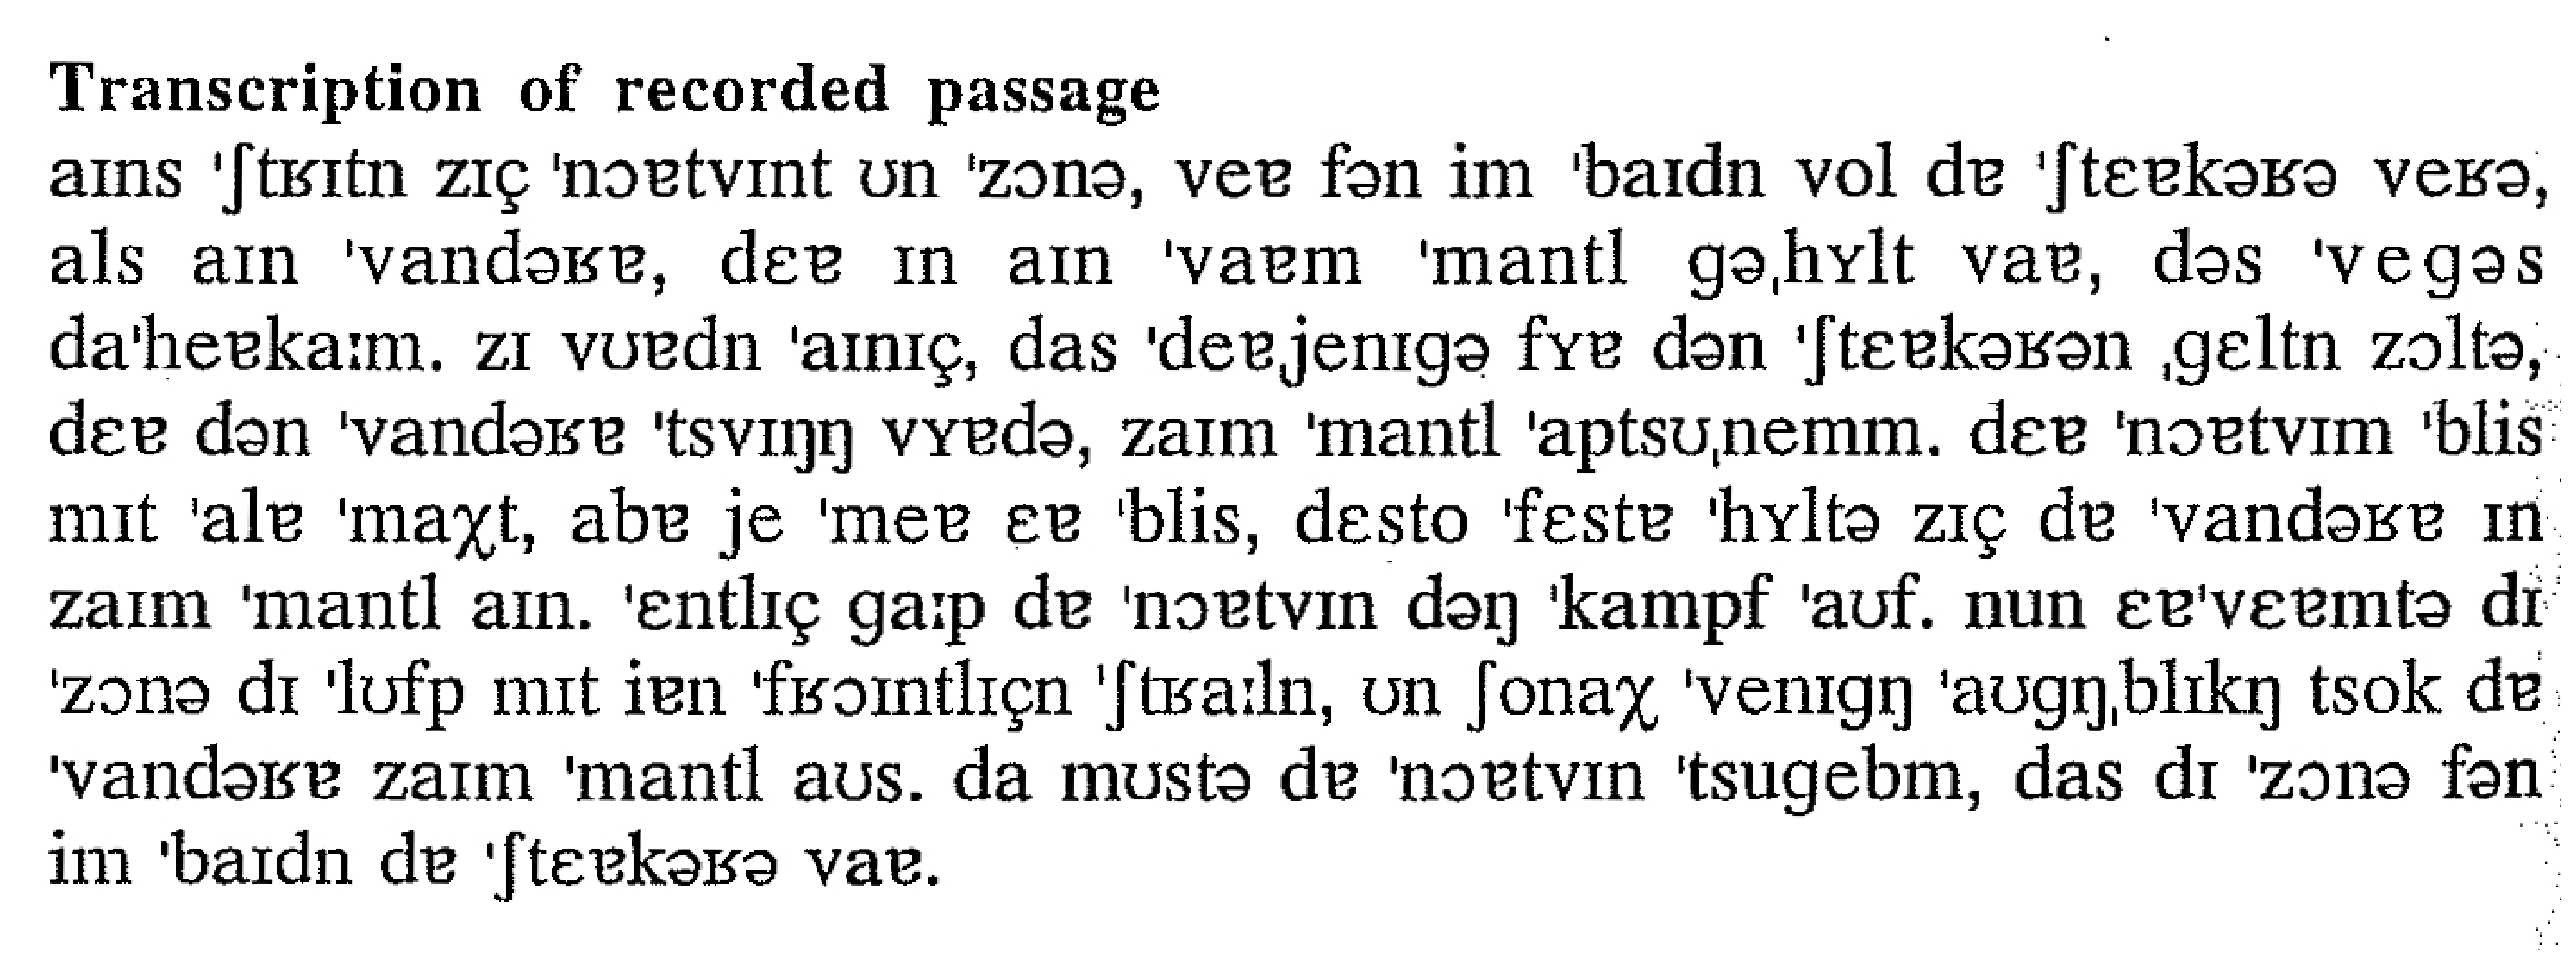
\includegraphics[scale=0.22]{material/04einststrittentranspompino}		
%	\end{figure}
\end{itemize}
	
	\begin{itemize}
		\item \href{run:material/04einststrittenaudio/04einststritten.wpl}{\textbf{SOUND}}
	\end{itemize}

	
\end{frame}


%%%%%%%%%%%%%%%%%%%%%%%%%%%%%%%%%%%%%%%%%%%%%%%%%%%%%%%

\iftoggle{ha-loesung}{
	\begin{frame}
\frametitle{Lösung}

Einst stritten sich Nordwind und Sonne, wer von ihnen beiden wohl der Stärkere wäre, als ein
Wanderer, der in einen warmen Mantel gehüllt war, des Weges daherkam. Sie wurden einig, dass
derjenige für den Stärkeren gelten sollte, der den Wanderer zwingen würde, seinen Mantel
abzunehmen. Der Nordwind blies mit aller Macht, aber je mehr er blies, desto fester hüllte sich der
Wanderer in seinen Mantel ein. Endlich gab der Nordwind den Kampf auf. Nun erwärmte die Sonne die
Luft mit ihrem freundlichen Strahlen, und schon nach wenigen Augenblicken zog der Wanderer seinen
Mantel aus. Da musste der Nordwind zugeben, dass die Sonne von ihnen beiden der Stärkere war.

\citep{Pompino95a}, \citep{Kohler99a}

\end{frame}
}


%%%%%%%%%%%%%%%%%%%%%%%%%%%%%%%%%%%%%%%%%%%%%%%%%%%%%%

\begin{frame}{\textipa{[ S l U s ]}}

	\begin{itemize}
		\item \textbf{VIDEO:} \href{run:material/04vocalcordssinging.mp4}{Vocal Cords}
	\end{itemize}
	
\end{frame}


%%%%%%%%%%%%%%%%%%%%%%%%%%%%%%%%%%%%%%%%%%%%%%%%%%%%%%%%%%%%%%%%
%%%%%%%%%%%%%%%%%%%%%%%%%%%%%%%%%%%%%%%%%%%%%%%%%%%%%%%%%%%%%%%%
\subsection{Abbildungen}
\begin{frame}[allowframebreaks]{Abbildungen}
	\small
		
		\begin{itemize}
			\item ABBILDUNG -- \gqq{Rousselots Apparat zur Aufzeichnung der Sprache} (Zugriff: 09.12.16): \url{https://de.wikipedia.org/wiki/Jean-Pierre\_Rousselot\#/media/File:Rousselots\_Apparat\_zur\_Aufzeichnung\_der\_Sprache.jpg}
			\item ABBILDUNG -- \gqq{Spektogramm \gq{Pronouncing}} (Autor: Rjanag, Zugriff: 20.12.16) \url{https://upload.wikimedia.org/wikipedia/commons/3/30/Pronouncing.PNG?uselang=de}
			\item ABBILDUNG -- Abbildung \gqq{IPA vowel chart} (CC BY-SA 3.0, Zugriff: 09.12.16) \url{https://en.wikipedia.org/w/index.php?curid=3368128}
			\item ABBILDUNG -- \gqq{Sagittalschnitt} (CC BY-SA 3.0, Zugriff: 09.12.16) \url{https://commons.wikimedia.org/w/index.php?curid=2615572}
		\end{itemize}	
	
\end{frame}

\subsection{Elektronische Quellen}
%\frame{
%\begin{multicols}{2}
%\frametitle{~}
%	\tableofcontents[currentsection]
%\end{multicols}
%}
%%%%%%%%%%%%%%%%%%%%%%%%%%%%%%%%%%%%%%%%%%%%%%%%%%%%%%%%%%%%%%%%

\begin{frame}[allowframebreaks]{Elektronische Quellen}
	\small
	
	\begin{itemize}
		\item VIDEO -- \gqq{Spoken Pirahã with subtitles} (Zugriff: 24.10.2013): \url{http://www.youtube.com/watch?v=SHv3-U9VPAs}
		\item LINK -- \gqq{Webseite der IPA} (Zugriff: 24.10.2013): \url{http://internationalphoneticassociation.org}
		\item LINK -- \gqq{Peter Ladefoged -- A Course in Phonetics} (Alle Laute zum Testen) (Zugriff: 24.10.2013):\\ \url{http://phonetics.ucla.edu/course/chapter1/chapter1.html}
		\item VIDEO -- \gqq{!Nama Clicks} (Zugriff: 24.10.2013): \url{http://www.youtube.com/watch?v=Ophrf64fxgA&list=PL6rcWnFnBuT7BEAex2IvI6l_bjLLycxaU}
		\item VIDEO -- \gqq{Anatomical Tutorial During Trans-Nasal Endoscopy} (Zugriff: 24.10.2012): \url{http://www.youtube.com/watch?v=wjRsa77u6OU}
		\item LINK -- \gqq{Interactive Sagittal Section} (Zugriff: 27.04.2016): \url{http://smu-facweb.smu.ca/~s0949176/sammy/}
		\item VIDEO -- \gqq{Vocal Cords up close while singing} (Zugriff: 24.10.2012): \url{http://www.youtube.com/watch?v=-XGds2GAvGQ}
	\end{itemize}
	
\end{frame}


